%%========================================================================
%% LaTeX sjabloon voor stage/projectrapport of bachelorproef
%%  HoGent Bedrijf en Organisatie
%%========================================================================

%%========================================================================
%% Preamble
%%========================================================================

\documentclass[pdftex,a4paper,12pt,twoside]{report}

% XXX: Let op: dit sjabloon is gemaakt om dubbelzijdig af te drukken
% Voor enkelzijdig, verwijder ``twoside'' hierboven.

%%---------- Extra functionaliteit ---------------------------------------

\usepackage[utf8]{inputenc}  % Accenten gebruiken in tekst (vb. é ipv \'e)
\usepackage{amsfonts}        % AMS math packages: extra wiskundige
\usepackage{amsmath}         %   symbolen (o.a. getallen-
\usepackage{amssymb}         %   verzamelingen N, R, Z, Q, etc.)
\usepackage[dutch]{babel}    % Taalinstellingen: woordsplitsingen,
                             %  commando's voor speciale karakters
                             %  ("dutch" voor NL)
\usepackage{eurosym}         % Euro-symbool €
\usepackage{geometry}
\usepackage{wrapfig}
\usepackage{graphicx}        % Invoegen van tekeningen
\graphicspath{ {img/} }
\usepackage{float}
\usepackage[pdftex,bookmarks=true]{hyperref}
                             % PDF krijgt klikbare links & verwijzingen,
                             %  inhoudstafel
\usepackage{listings}        % Broncode mooi opmaken
\usepackage{multirow}        % Tekst over verschillende cellen in tabellen
\usepackage{rotating}        % Tabellen en figuren roteren
\usepackage{natbib}          % Betere bibliografiestijlen
\usepackage{fancyhdr}        % Pagina-opmaak met hoofd- en voettekst

\usepackage[T1]{fontenc}     % Ivm lettertypes
\usepackage{lmodern}
\usepackage{textcomp}
\usepackage[intoc]{nomencl}
\usepackage{url}
\makenomenclature


%\usepackage{hyperref}        %hyperlinks

\usepackage{lipsum}          % Voor vultekst (lorem ipsum)

%%---------- Layout ------------------------------------------------------

% hoofdingen, enz.
\pagestyle{fancy}
% enkel hoofdstuktitel in hoofding, geen sectietitel (vermijd overlap)
\renewcommand{\sectionmark}[1]{}

% lijn, wordt gebruikt in titelpagina
\newcommand{\HRule}{\rule{\linewidth}{0.5mm}}

% Leeg blad
\newcommand{\emptypage}{
\newpage
\thispagestyle{empty}
\mbox{}
\newpage
}

% Gebruik een schreefloos lettertype ipv het "oubollig" uitziende
% Computer Modern
\renewcommand{\familydefault}{\sfdefault}

%afkortingshizzle
\renewcommand{\nomname}{Lijst van afkortingen}

% Commando voor invoegen Java-broncodebestanden (dank aan Niels Corneille)
% Gebruik: \codefragment{source/MijnKlasse.java}{Uitleg bij de code}
\newcommand{\codefragment}[2]{ \lstset{%
  language=java,
  breaklines=true,
  float=th,
  caption={#2},
  basicstyle=\scriptsize,
  frame=single,
  extendedchars=\true
}
\lstinputlisting{#1}}

%%---------- Documenteigenschappen ---------------------------------------
%% Vul dit aan met je eigen info:

% Je eigen naam
\newcommand{\student}{Thomas Verelst}

% De naam van je lector, begeleider, promotor
\newcommand{\promotor}{Jens Buysse}

% De naam van je co-promotor
\newcommand{\copromotor}{Daan De Jaeghere}

% Indien je bachelorproef in opdracht van een bedrijf of organisatie
% geschreven is, geef je hier de naam.
%\newcommand{\instelling}{---}

% De titel van het rapport/bachelorproef
\newcommand{\titel}{De mogelijkheden van Augmented Reality op handheld toestellen in het onderwijs}

% Datum van indienen
\newcommand{\datum}{27 mei 2016}

% Faculteit
\newcommand{\faculteit}{Faculteit Bedrijf en Organisatie}

% Soort rapport
\newcommand{\rapporttype}{Scriptie voorgedragen tot het bekomen van de graad van\\Bachelor in de toegepaste informatica}

% Academiejaar
\newcommand{\academiejaar}{2015-2016}

% Examenperiode
%  - 1e semester = 1e examenperiode
%  - 2e semester = 2e examenperiode
%  - tweede zit = 3e examenperiode
\newcommand{\examenperiode}{2e examenperiode}

%%========================================================================
%% Inhoud document
%%========================================================================

\begin{document}

%%---------- Front matter ------------------------------------------------
%% Het voorblad - Hier moet je in principe niets wijzigen.

\begin{titlepage}
  \newgeometry{top=2cm,bottom=1.5cm,left=1.5cm,right=1.5cm}
  \begin{center}

    \begingroup
    \rmfamily
    
\includegraphics[width=2.5cm]{img/HG-beeldmerk-woordmerk}\\[.5cm]
    \faculteit\\[3cm]
    \titel
    \vfill
    \student\\[3.5cm]
    \rapporttype\\[2cm]
    Promotor:\\
    \promotor\\
    Co-promotor:\\
    \copromotor\\[2.5cm]
%    Instelling: \instelling\\[.5cm]
    Academiejaar: \academiejaar\\[.5cm]
    \examenperiode
    \endgroup

  \end{center}
  \restoregeometry
\end{titlepage}

% Schutblad

\emptypage


\begin{titlepage}
  \newgeometry{top=5.35cm,bottom=1.5cm,left=1.5cm,right=1.5cm}
  \begin{center}

    \begingroup
    \rmfamily
    \faculteit\\[3cm]
    \titel
    \vfill
    \student\\[3.5cm]
    \rapporttype\\[2cm]
    Promotor:\\
    \promotor\\
    Co-promotor:\\
    \copromotor\\[2.5cm]
%    Instelling: \instelling\\[.5cm]
    Academiejaar: \academiejaar\\[.5cm]
    \examenperiode
    \endgroup

  \end{center}
  \restoregeometry
\end{titlepage}


\begin{abstract}
% TODO: De "abstract" of samenvatting is een kernachtige (max 1 blz. voor een
% thesis) synthese van het document. In ons geval beschrijf je kort de
% probleemstelling en de context, de onderzoeksvragen, de aanpak en de
% resultaten.
Augmented Reality is de laatste jaren een hot topic. Het is een technologie waarbij beelden van de werkelijkheid verrijkt worden met virtuele elementen. Augmented Reality is geen sciencefiction meer, maar is een technologie van deze tijd en deze wereld. Tegenwoordig kunnen op elke smartphone of tablet (handhelds) uitgerust met een camera applicaties ge\"installeerd worden die gebruik maken van Augmented Reality. Handhelds raken stilaan ge\"integreerd in scholen en daarbij wordt ook Augmented Reality toegankelijker in de klas. Deze scriptie gaat op zoek naar een antwoord op de vraag: Waarom Augmented Reality op handhelds in het onderwijs en wat zijn de mogelijkheden? Eerst volgt een algemene kadering rond Augmented Reality, vervolgens de mogelijkheden en het nut van de technologie in het onderwijs. Als case study werd een concrete les voorbereid en uitgevoerd. De voorbereiding, observaties en reacties worden uitgebreid besproken. Uit het literatuuronderzoek in combinatie met de case study concludeert het document dat Augmented Reality een goede ondersteuning kan bieden aan lessen en dat er tal van mogelijkheden bestaan om de technologie aan te wenden.   \\

\end{abstract}

\chapter*{Voorwoord}
\label{ch:voorwoord}

% TODO: Vergeet ook niet te bedanken wie je geholpen/gesteund/... heeft
Naast mijn passie voor alles wat met computers te maken heeft, ben ik ook zeer ge\"interesseerd in onderwijs. Ik ben dan ook zeer blij dat ik deze twee heb kunnen combineren in deze scriptie. De scriptie had niet mogelijk kunnen zijn zonder een aantal mensen en ik had deze dan ook graag bedankt.\\

Mijn promotor Jens Buysse verzorgde een goede begeleiding. Wanneer ik in het begin twijfelde aan het onderwerp gaf meneer Buysse me de motivatie om verder te werken. \\

Mijn co-promotor Daan De Jaeghere voorzag de mogelijkheid om een concrete les uit te werken. De hoeveelheid tijd dat Daan vrijmaakte om te overleggen en de samen de les voor te bereiden was ongelofelijk. Ik ben hem dan ook z\'e\'er dankbaar. \\

Verder wil ik nog mijn vader bedanken voor het nalezen van de scriptie en de geboden steun. Ook mijn collega's op stage Jeroen Cornelis en Micha\"el Van Neygen boden telkens een luisterend oor en gaven steun.

\tableofcontents

% Als je een lijst van afkortingen of termen wil toevoegen, dan hoort die
% hier thuis. Gebruik bijvoorbeeld de ``glossaries'' package.

%%---------- Kern --------------------------------------------------------

\chapter{Inleiding}
\label{ch:inleiding}

Heel veel mensen komen in contact met Augmented Reality zonder dit te beseffen. Op bijna iedere handheld staat wel een applicatie die gebruik maakt van Augmented Reality. Zo gebruikt snapchat filters waarbij gebruikers allerlei manipulaties kunnen uitvoeren op foto's \citep{Snapchat}. De Google Translate app implementeerde begin vorig jaar Augmented Reality waardoor het nu mogelijk is om tekst te vertalen aan de hand van een foto \citep{GoogleTrans}. Augmented Reality heeft ondertussen al enorm veel toepassingen en door de opkomst van de smartphones en tablets is het toegankelijker dan ooit  \citep{tablets}.\\

De opkomst van de tablets en smartphones is ook het onderwijs niet ontgaan. Vele scholen stellen al tablets ter beschikking aan hun leerlingen en leerkrachten voor educatieve doeleinden. Sommige scholen gaan zelfs verder en verplichten de aankoop van een tablet \citep{ipadschool}. Vele leerkrachten zijn continue op zoek naar nieuwe manieren om hun lessen te innoveren, interactief of leerrijker te maken. Ook de onderwijscompetenties van de Vlaamse overheid sturen aan op moderne ICT integratie.  Augmented Reality sluit hierbij perfect aan. De mogelijkheden voor het onderwijs zijn talrijk en er bestaan ook tal van applicaties voor handhelds die ondersteuning kunnen bieden aan leerkrachten \citep{eduapps}. Naast de extra waarde die Augmented Reality aan de leerstof kan toevoegen krijgen ook leerlingen de kans om zich te ontwikkelen op vlak van ICT. 




\section{Probleemstelling \& Onderzoeksvragen}
\label{sec:onderzoeksvragen}

Deze scriptie probeert een antwoord te formuleren op de volgende onderzoeksvragen:

\begin{quote}
Waarom Augmented Reality op handhelds in het onderwijs en wat zijn de mogelijkheden? 
\end{quote}

Om een antwoord op deze vraag te vinden onderzoek ik wat Augmented Reality is en bespreek ik enkele belangrijke toepassingen. Vervolgens zal de huidige plaats van en handhelds van AR en handhelds in het onderwijs aan bod komen en ga ik in op de renenen om AR aan te wenden op een educatieve manier. \\

Als case study wordt een concrete les voorbereid en gegeven met behulp van Augmented Reality. In het verleden gaven verschillende studies aan dat de technologie nog niet rijp genoeg was en technische problemen te vaak irritaties konden veroorzaken \citep{aredu}, \citep{dunleavy2009affordances}, \citep{kerawalla2006}. De bedoeling van deze case study is om aan te tonen dat Augmented Reality effectief gebruikt kan worden in hedendaags onderwijs en de technologie hiervoor beschikbaar is op handhelds.  
\chapter{Augmented Reality}
\label{ch:AR}

\section{Introductie}
\subsection{Definitie}
\label{sec:def}
Hoewel Augmented Reality alom aanwezig is, bevat het Van Dale woordenboek tot op heden nog geen definitie voor Augmented Reality.  Vorig jaar haalde \cite{degrande} de definitie van AR aan. Deze definitie kwam van het online woordenboek Merriam-Webster \citep{merriam} en is nog steeds dezelfde:

 \begin{quote}
  An enhanced version of reality created by the use of technology to overlay digital information on an image of something being viewed through a device (as a smartphone camera).
 \end{quote}

Na vertaling naar het Nederlands wordt dit:

 \begin{quote}
  Een meer uitgebreide versie van realiteit gecre\"eerd door het gebruik van technologie die informatie plaatst bovenop een beeld bekeken door een toestel (zoals een smartphone camera).
 \end{quote}
\begin{itemize}
  \item \textbf{Meer uitgebreide versie van de realiteit}: Het doel van Augmented Reality is om een meerwaarde te geven aan de realiteit met virtuele uitbreidingen.
	\item \textbf{Gecre\"eerd door het gebruik van technologie}: Zonder technologie is er geen virtueel aspect en kunnen we dus niet spreken van Augmented Reality.
	\item \textbf{Plaatsen van informatie}: De meerwaarde gegeven door Augmented Reality is een toevoeging van informatie aan een waarneming. Deze meerwaarde kan zowel visueel als audio zijn.
	\item \textbf{Een beeld}: Voor Augmented Reality is er uiteraard een beeld om te bewerken nodig.
	\item \textbf{Bekeken door een toestel}: Om de toevoegingen van digitale elementen te kunnen doen moet een beeld getoond kunnen worden. Hoewel dit inderdaad vaak door een toestel met een camera is, kunnen dit ook gerust projecties zijn. Dit deel van de definitie is enkel van toepassing voor see-through Augmented Reality, besproken in sectie \ref{sec:spatial}, en is overbodig voor de overkoepelende Augmented Reality term.
\end{itemize}

Kortom, Augmented Reality is een breed begrip en kan ook eerder gezien worden als een concept in plaats van een technologie. De mogelijkheden zijn ongelimiteerd en naarmate algemene technologi\"en vooruitgang boeken zal Augmented Reality ongetwijfeld mee groeien.	\\

\subsection{See-through en spatial Augmented Reality}
\label{sec:spatial}
Augmented Reality is onderverdeeld in twee takken. Enerzijds is er de spatial AR, anderzijds is er de see-through AR \citep{milgram1995augmented}.

\begin{wrapfigure}{r}{0.4\textwidth}
\vspace{-15pt}

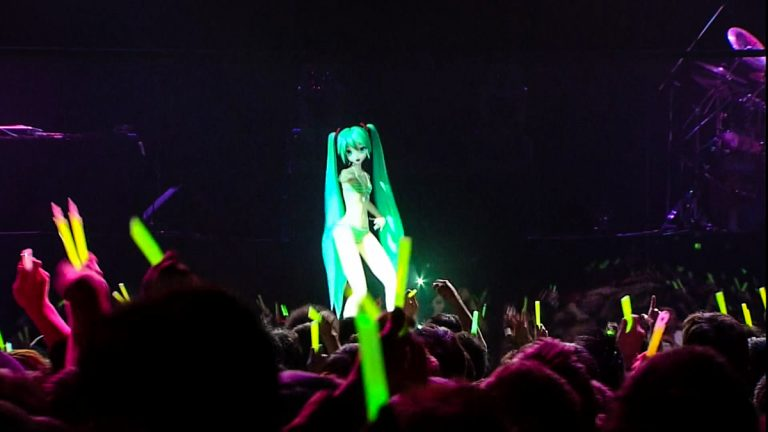
\includegraphics[scale=0.22]{miku} 
\caption{Optreden Hatsune Miku \citep{miku}}  \label{fig:miku}
\vspace{-20pt}
\end{wrapfigure}

\paragraph{Spatial AR}
Hieronder verstaan we alle computer gegenereerde informatie die rechtstreeks ge\"injecteerd wordt in de omgeving van de gebruiker. Zo vallen bijvoorbeeld optredens gegeven door hologrammen zoals Hatsune Miku (figuur \ref{fig:miku}) onder spatial AR. Op handheld devices komt deze vorm van Augmented Reality niet vaak voor. Hiervoor is ook andere hard- en software voor nodig dan voor see-through AR.

\paragraph{See-through AR}
Vooraleer er toegevoegde informatie waargenomen kan worden moet bij see-through AR een gebruiker eerst ergens doorkijken. Op handhelds kan dit de via camera van het toestel. Het apparaat toont dan het bewerkte beeld op het scherm. Dit is de courantste vorm van Augmented Reality mits tegenwoordig bijna iedere handheld wel een camera heeft en geen projector. Wanneer in deze scripte verwezen wordt naar Augmented Reality wordt er see-through AR bedoeld wordt. Indien dit niet het geval is zal dit expliciet vermeld staan.


\subsection{Virtual Reality}
Naast Augmented Reality komt Virtual Reality vaak voor in de media.	De technologi\"en liggen dicht bij elkaar maar mogen zeker niet met elkaar verward worden. Zoals eerder besproken in sectie \ref{sec:def} voegt Augmented Reality virtuele elementen toe aan een bestaande realiteit. Virtual Reality daarintegen maakt een volledig virtuele omgeving bedoeld om een echte situatie of werkelijkheid te simuleren en dit voornamelijk met beeld en geluid. Virtual Reality heeft vooral zijn plaats gevonden in de wereld van ontspanning (games, films, ...) maar wordt ook gebruikt voor andere doeleinden waaronder het trainen van piloten of vrachtwagenchauffeurs.

\subsubsection{Gelijkenissen}
Beide technologi\"en zouden even goed uit een sciencefiction kunnen komen en ze kunnen geassocieerd worden met head-mounted displays. Ze cre\"eeren beiden virtuele elementen en beiden hebben als doel de gebruiker te verrijken met deze virtualisaties. Beiden hebben ze ontelbaar veel mogelijkheden voor zowel recreatieve als professionele doeleinden.

\subsubsection{Verschillen}
Zoals eerder vermeld zijn in Virtual Reality alle beelden gegenereerd door een computer. In Augmented Reality is er altijd een element van werkelijkheid. Een computer kan die realiteit niet sturen of be\"invloeden. Een ander belangrijk verschil is de vereiste apparatuur. Augmented Reality kan gebruikt worden op zowat elke handheld, laptop of computer. Voor Virtual Reality is er nog steeds speciale apparatuur nodig zoals een head-mounted display. Dit zou wel eens een reden kunnen zijn waarom Augmented Reality zich breder en sneller kan ontwikkelen.
  
\subsection{Beknopte historiek}
\begin{wrapfigure}{r}{0.35\textwidth}
\vspace{-15pt}
\caption{Head-mounted displays \citep{history2}} \label{fig:sutherlandimg}
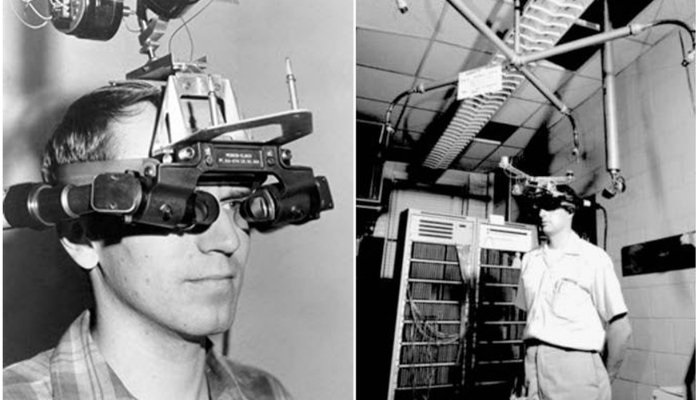
\includegraphics[scale=0.25]{sutherland}
\vspace{10pt}
\end{wrapfigure}

\paragraph{1968} Alhoewel er van de term Augmented Reality nog lang geen sprake was, waren er in de loop van de twinstige eeuw al enkele individuen bezig met het concept. Een van de eerste was Ivan Sutherland, een Professor aan Harvard University. In 1968 ontwierp hij een model waar tegenwoordig veel Augmented en Virtual Reality toepassingen mee werken: de head-mounted display. Doordat de technologie nog zeer gelimiteerd was, was de display te zwaar om door een mens gedragen te worden. Dit is te zien in figuur \ref{fig:sutherlandimg}. Het toestel toonde zeer eenvoudige wireframe modellen.

\paragraph{1992} In 1992 gebruiken Tom Caudell en David Mizell voor het eerst de term Augmented Reality. Zij waren bezig met het schrijven van complexe software. Deze software had als doel om het bouwproces van vliegtuigen te assisteren. Op datzelfde ogenblik waren ook twee andere teams bezig met het ontwikkelen van AR-systemen \citep{history}. \`E\`en van de teams werkte voor de United States Airforce een systeem uit dat hielp om bepaalde taken uit te voeren \citep{rosenberg}.
 Het andere team maakte een printer waarbij de instructies werden geprojecteerd en een gebruiker de machine kon gebruiken zonder handleiding \citep{history}.

\paragraph{1999} Omdat AR dure technologie en zware computers vereiste, was AR niet toegankelijk voor het grote publiek. AR bleef sinds het onstaan vrijwel exclusief tot onderzoek en laberatoria beperkt bleef. Tot 1999. In '99 kondigden Hirokazu Kato en Mark Billinghurst \cite{artoolkit} aan. Met ARToolKit konden virtuele elementen toegevoegd worden aan een video stream. ARToolkit wordt verder besproken in sectie \ref{sec:tools}.

\paragraph{2008}Toen er ondertussen al een hele lijst aan AR toepassing ontwikkeld was \citep{history2}, kwam in 2008 de eerste app voor smartphones. Wikitude toont gebruikers info over nabije nuttige plaatsen. De app was oorspronkelijk enkel voor android ontwikkeld. Door het grote success was deze al snel ook beschikbaar op de andere platformen.

\paragraph{2013} Het waarschijnlijk meest bekende AR product kwam in 2013 op de markt, Google Glass. Hierover meer in sectie \ref{sec:googleglass}.
\newpage
\begin{wrapfigure}{l}{0.3\textwidth}

\label{fig:htcvive}
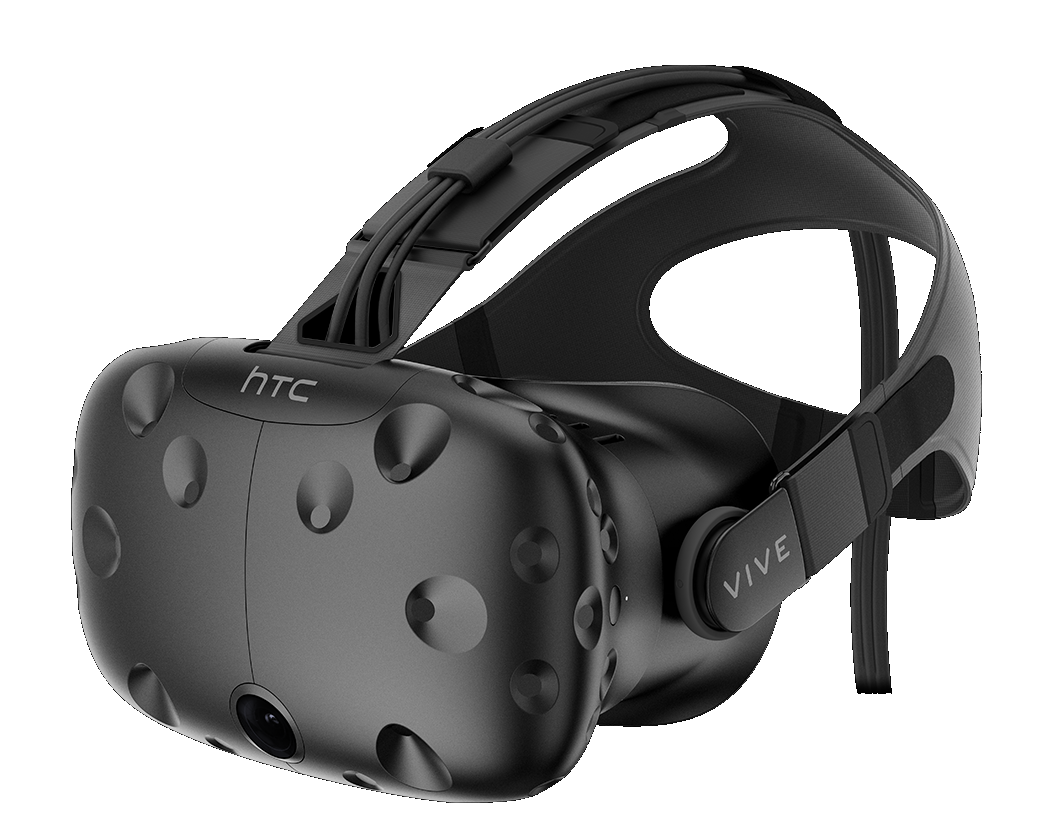
\includegraphics[scale=0.15]{htcvive.png}
\caption{Htc vive headset \citep{htcvive}}

\end{wrapfigure}

\paragraph{2016} Oculus en HTC brachten in 2016 beiden Virtual Reality headsets uit op de markt \citep{oculus}, \citep{htcvive}. Hoewel dit over Virtual en niet Augmented reality gaat, is de release van deze headsets ongetwijfeld een mijlpaal voor het commercialiseren van deze technologi\"en. Met deze headsets kunnen gebruikers in een volledig virtuele wereld stappen. De headsets blijken een enorm succes te zijn. Zo kondigde HTC begin mei aan voorlopig geen bestellingen meer op te nemen in de Verenigde Staten door overweldigend succes \citep{htcsucces}. \\

\paragraph{2016} Unity organiseerde in februarie het evenement Vision VR/AR Summit. Dit evenement was enkel en alleen op VR en AR gericht. Unity werkte hiervoor samen met enkele andere grote spelers waaronder Oculus, Microsoft, Vuforia, Sony, Steam en Google \citep{summit}. Ontwikkelaars, artiesten en iedereen die iets te maken heeft met Augmented of Virtual Reality kon hier zijn product of project tentoonstellen. \\

 Augmented Reality blijft groeien en nieuwe toepassingen kennen. Door het enorm aantal stijgend gebruikers van smartphones zijn apps razend populair geworden \citep{smartpop}. Tal van bedrijven zoals Augment, Layar en Aurasma leveren AR services op mobile platforms maar ook met opensource toolkits en frameworks zoals ARToolkit kunnen ook programmeurs aan de slag. 


\section{Werking Augmented Reality}

  \subsection{Tracking}
	\label{sec:tracking}
	Het toestel voor Augmented Reality moet, voordat het iets kan tonen, weten wat er getoond moet worden en waar. Hiervoor moeten de beelden die waargenomen worden door het toestel, informatie bevatten op basis waarvan het toestel dit kan afleiden. Dit probleem staat beter bekend als tracking. In het geval van Augmented Reality wordt vaak gebruik gemaakt van marker-based tracking. Bij marker-based tracking identificeert het apparaat patronen met behulp van de afbeelding herkenning. Deze patronen worden dan ge\"identificeerd door het toestel waarna het weet wat er getoond moet worden. Dit komt neer op hetzelfde principe als QR codes of gewone barcodes, waarbij een patroon data bevat die een computer kan interpreteren. Dankzij geadvanceerde technologi\"en in het domein van computervisie kunnen ook complexe afbeeldingen of voorwerpen als patroon herkend worden, zodat Augmented Reality niet afhangt van zwart-wit codes. \\
	
	\subsection{Beeld}
	Op smartphones en tablets worden de toepassingen van Augmented Reality vrijwel altijd bekeken op het scherm van het toestel. Indien de getoonde stroom van beelden niet vloeiend gaat dan kan dit erg storend zijn voor de gebruiker van de applicatie. De beelden die getoond worden door AR applicaties zijn over het algmeen 3D modellen. Deze worden op het scherm getoond, maar het scherm is 2D. Het proces dat 3D beelden converteert naar 2D heet rendering. Nadat de beelden op het gebruikte apparaat zijn waargenomen door de camera en vervolgens bewerkt door de software, toont het apparaat deze op het scherm. Hoe vlot het apparaat de stroom van beelden toont kan gemeten worden in frames per seconde (fps). Naar gelang de hardware en software dat het apparaat gebruikt, kunnen er fluctuaties zijn in het aantal fps. Hoe groter het aantal fps, hoe vlotter de video. Als de gebruiker dus te maken krijgt met schokkende beelden dan is dit te vaak wijten aan een laag aantal fps . Doorheen de jaren zijn smartphones en tablets steeds uitgerust met betere hardware en is dit niet zo'n groot probleem meer. Er moet wel nog steeds rekening mee worden gehouden.\\
	
	In geval van spatial AR worden beelden getoond met behulp van projectoren. Vaak worden ook cameras gebruikt zodat het apparaat kan bepalen waar de projectie precies moet komen.

\section{Toepassingen Augmented Reality}
	
\subsection{Google Glass}
\label{sec:googleglass}

\begin{wrapfigure}{r}{0.35\textwidth}

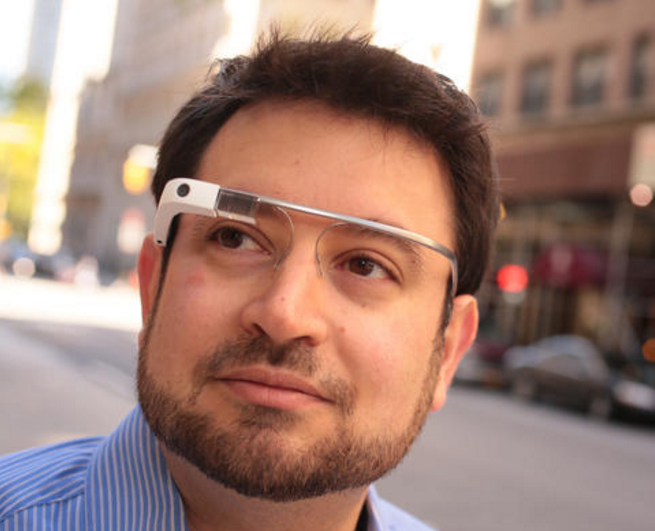
\includegraphics[scale=0.25]{googleAan.png}
\caption{Google Glasses \citep{ggFotoAan}} 
\end{wrapfigure}

Google kondigde voor het eerst hun Google Glass project in 2012 \citep{ggannounce}. Google Glass is een head-mounted display met een ingebouwde computer in de vorm van een bril. Een gebruiker kan het toestel besturen met zijn stem of een touchpad aan de zijkant van de bril. Om de virtualisaties te kunnen tonen aan een gebruiker projecteert het toestel beelden rechtstreeks op de retina van het oog. De bril kan beschouwd worden als een handsfree smartphone. Met Augmented Reality kunnen alle beelden via de bril bewerkt worden.\\

In 2013 werd Google Glass beschikbaar voor het publiek \citep{ggHistory}. De mogelijkheden van de Google Glass leken eindeloos maar er kwam veel kritiek. Zo was het in verschillende Amerikaanse staten niet toegelaten om de bril te dragen tijdens het rijden. Ook de inbreuk op de privacy werd een veelbesproken thema. In veel banken, ziekenhuizen, cinema's en andere publieke plaatsen werd Google Glass verbannen. Een van de redenen hiervoor is dat een gebruiker te eenvoudig opnames kan maken van zaken die onder auteursrecht vallen of gevoelige informatie bevatten. \\

Begin 2015 koos Google ervoor om de verkoop van Google Glass stop te zetten. Google kondigde aan dat teleurstellende verkoopcijfers de belangrijkste reden was voor deze beslissing, hoewel de controversie rond het product hier ook zeker heeft meegespeeld \citep{ggFail}. Wel kondigde Google aan niet op te geven en een nieuw project te zijn gestart voor de ontwikkeling van een nieuw product gebaseerd op Google Glass.\\

Hoewel de commercialisatie van Google Glass geen succes was zijn er toch veel toepassingen waarin de bril zijn nut bewijst \citep{ggUses}. Zo zijn er dokters die opereren met behulp van Google Glass. De bril kan extra cruciale informatie aan de chirurg tonen zonder dat hij moet wegkijken van de patient, ge\"illustreerd in figuur \ref{fig:googleAan}. Ook bij de politie en in militaire operaties is de bril al ingezet geweest. Zo kan er in real-time extra informatie getoond worden aan de agenten en soldaten zonder dat zij moeten wegkijken van hun doel. \\


\begin{figure}[H]
\begin{center}
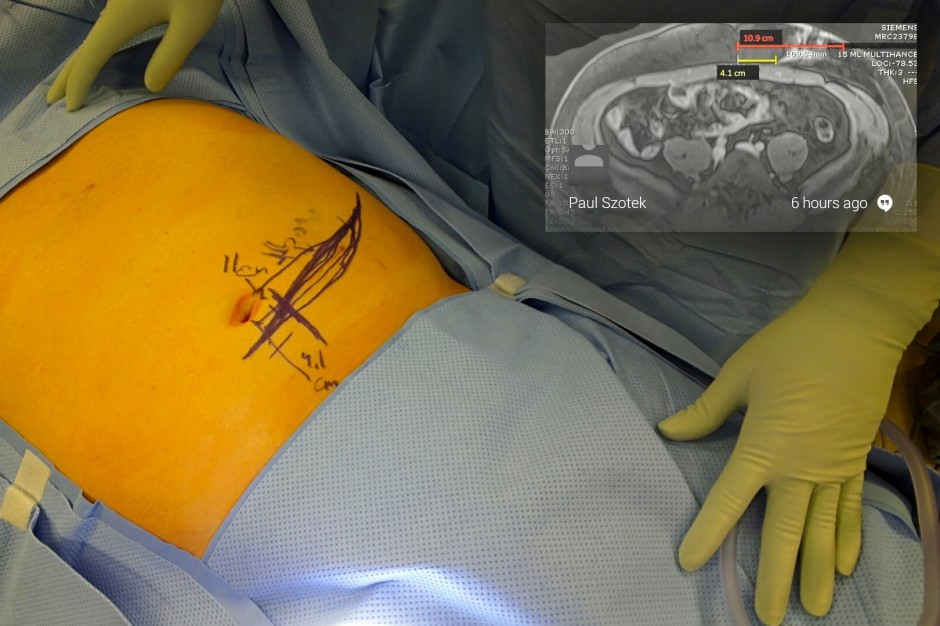
\includegraphics[scale=0.30]{googleIn.jpg}	
\end{center}
\caption{Voorbeeld van een beeld kijkend door Google Glass \citep{ggFotoIn}} \label{fig:googleAan}
\end{figure}


\begin{wrapfigure}{r}{0.3\textwidth}
\vspace{-5pt}
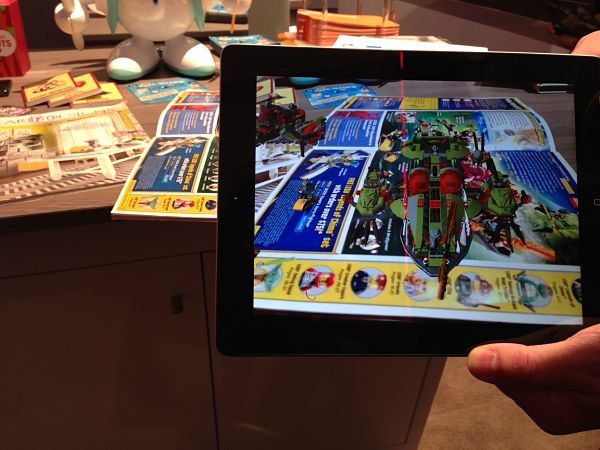
\includegraphics[scale=0.22]{lego.jpg}
\caption{Lego advertentie met AR\citep{legoFoto}} \label{fig:lego}

\end{wrapfigure}


\subsection{Retail \& Advertenties}
De opkomst van Augmented Reality is ook de retail sector niet ontgaan. Al in 2009 lanceerde lego Augmented Reality in hun winkels \citep{lego}. Klanten kunnen een doos voor een camera houden, waarna op een scherm te zien is wat ze met de inhoud van de doos kunnen bouwen. Als klanten de doos draaien, roteert het model mee. Ondertussen kan dit ook al met een gewone brochure op een smartphone of een tablet zoals te zien in figuur \ref{fig:lego}. Ondertussen zijn vele andere bedrijven Augmented Reality beginnen gebruiken. Zo lanceerde IKEA ondertussen ook al een applicatie voor handhelds die gebruikt maakt van AR. Met deze applicatie kunnen gebruikers voorwerpen uit de IKEA catalogus in hun eigen omgeving plaatsen op hun toestel \citep{ikea}. Vooral met de explosieve groei van online winkelen \citep{webshops} lijkt deze technologie aantrekkelijk om klanten te overtuigen.\\

Er is onderzocht geweest of het gebruik van Augmented Reality in winkels ook wel effectief een impact heeft op het gedrag van de klant \citep{cuomo2015augmented}. Uit dit onderzoek werd besloten dat AR wel degelijk extra informatie en een betere ervaring aan de klant kan bieden waardoor de verkoopcijfers stijgen.

\subsection{Tools en Applicaties}
\label{sec:tools}
Er bestaan ondertussen een hele reeks van tools en applicaties, zowel gratis als betalend, waarmee gebruikers aan de slag kunnen met Augmented Reality. Een kleine selectie populaire applicaties komt hier aan bod.

\subsubsection{ARToolkit}
ARToolkit is een software development kit dat programmeurs kan helpen om Augmented Reality applicaties te programmeren. ARToolkit bied verschillende SDK's aan voor de populairste platformen. Op desktop ondersteunt de toolkit zowel Linux, OS X als Windows en op mobile zowel Android en iOS. De toolkit biedt een waaier van mogelijkheden aan waaronder verschillende soorten tracking en integratie met andere relevante software als Unity3D en OpenSceneGraph. \\

ARToolkit is ongetwijfeld een project dat enorm heeft bijgedragen aan de toegankelijkheid en het succes van Augmented Reality. In 1999 werd ARToolkit voor het eerst publiekelijk voorgesteld. Dit was ook de eerste keer dat een werkend AR-systeem gezien werd buiten een laboratium in de Verenigde Staten \citep{artoolkit}. Na de release van ARToolkit v1.0 in 2001 door het bedrijf ARToolworks duurde het niet lang voor de eerste applicaties en projecten naar boven kwamen. In 2002 al introduceerde HITLab NZ de Magic Book, een project dat gebruik maakte van ARToolkit \citep{billinghurst2001magicbook}. Doorheen de jaren bleef het project onderhouden en kwamen releases voor verschillende populaire en nieuwe platforms. In 2014 bereikte de tool 650.000 downloads \citep{artoolkit}.


\subsubsection{Layar}
Een van de eerste bedrijven dat zich specialiseerde in Augmented Reality op handhelds is Layar, opgericht in 2009. Zij ontwikkelden het gelijknamige product Layar. Hun product werd al snel populair omdat zij als een van de eerste AR bedrijven in staat waren om eender welke foto of afbeelding te gebruiken als tracker \citep{layarnumbers}. Dat een tracker onder meer een flyer of poster kon zijn, wekte plots veel interessanter bij marketing en retail. Hoort u liever de CEO zelf van het bedrijf zelf uitleg geven over de applicatie? Scan dan figuur \ref{fig:layar} met de Layar app! De Layer app maakt gebruik van een browser waarin Augmented Reality trackers kunnen toegevoegd worden. Deze trackers krijgen de toepasselijke naam layer. Het scannen van layers triggert bepaalde acties zoals het weergeven van extra informatie op flyers, het doorlinken naar een website of het afspelen van een video. \\

\begin{wrapfigure}{r}{0.2\textwidth}
\vspace{-30pt}
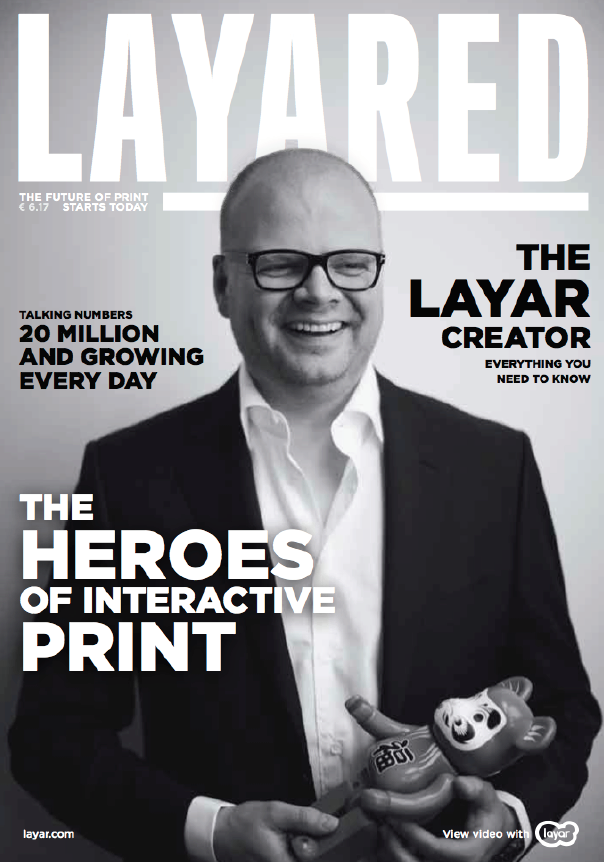
\includegraphics[scale=0.35]{layar}
\label{fig:layar}
\caption{Layar \citep{layarFoto}} \label{fig:layar}
\vspace{-30pt}
\end{wrapfigure}


In 2014 werd Layar overgenomen door een concurerend bedrijf Blippar. Na de fusie werkte Blippar samen met meer dan 5.000 merken en 100.000 individuele gebruikers \citep{blippar}. Layar is ondertussen een van de meest gebruikte AR applicaties. De app is al meer dan 40.000.000 keer gedownload en er zijn meer dan 500.000 layers geupload in de applicatie \cite{layarnumbers}. 



\subsubsection{Augment}
Augment is een bedrijf, begonnen in 2011, dat zich toespitst op see-though AR, specifiek in het visualiseren van 3D-modellen. Hun product is een augmented reality platform waar gebruikers 3D-modellen kunnen uploaden, delen en visualiseren. Het uploaden van modellen gebeurt via hun website of desktop applicatie. Voor het delen en visualiseren is er een applicatie voor handhelds, zowel Android als iOS. Naast 3D modellen kunnen gebruikers ook trackers uploaden en koppelen aan een model. Een van de sterke punten van Augment, net zoals bij Layar, is dat deze trackers een foto, tekening of code kunnen zijn. Wanneer iemand deze tracker scant met de Augment mobiele applicatie, verschijnt het model bovenop de tracker. Gebruikers kunnen ook in de Augment bibliotheek modellen opzoeken en oproepen zonder het gebruik van een tracker. In deze bibliotheek staan alle modellen die eerder zijn ge\"upload en beschikbaar zijn gesteld voor het publiek. \\

\begin{wrapfigure}{r}{0.3\textwidth}
\vspace{-15pt}
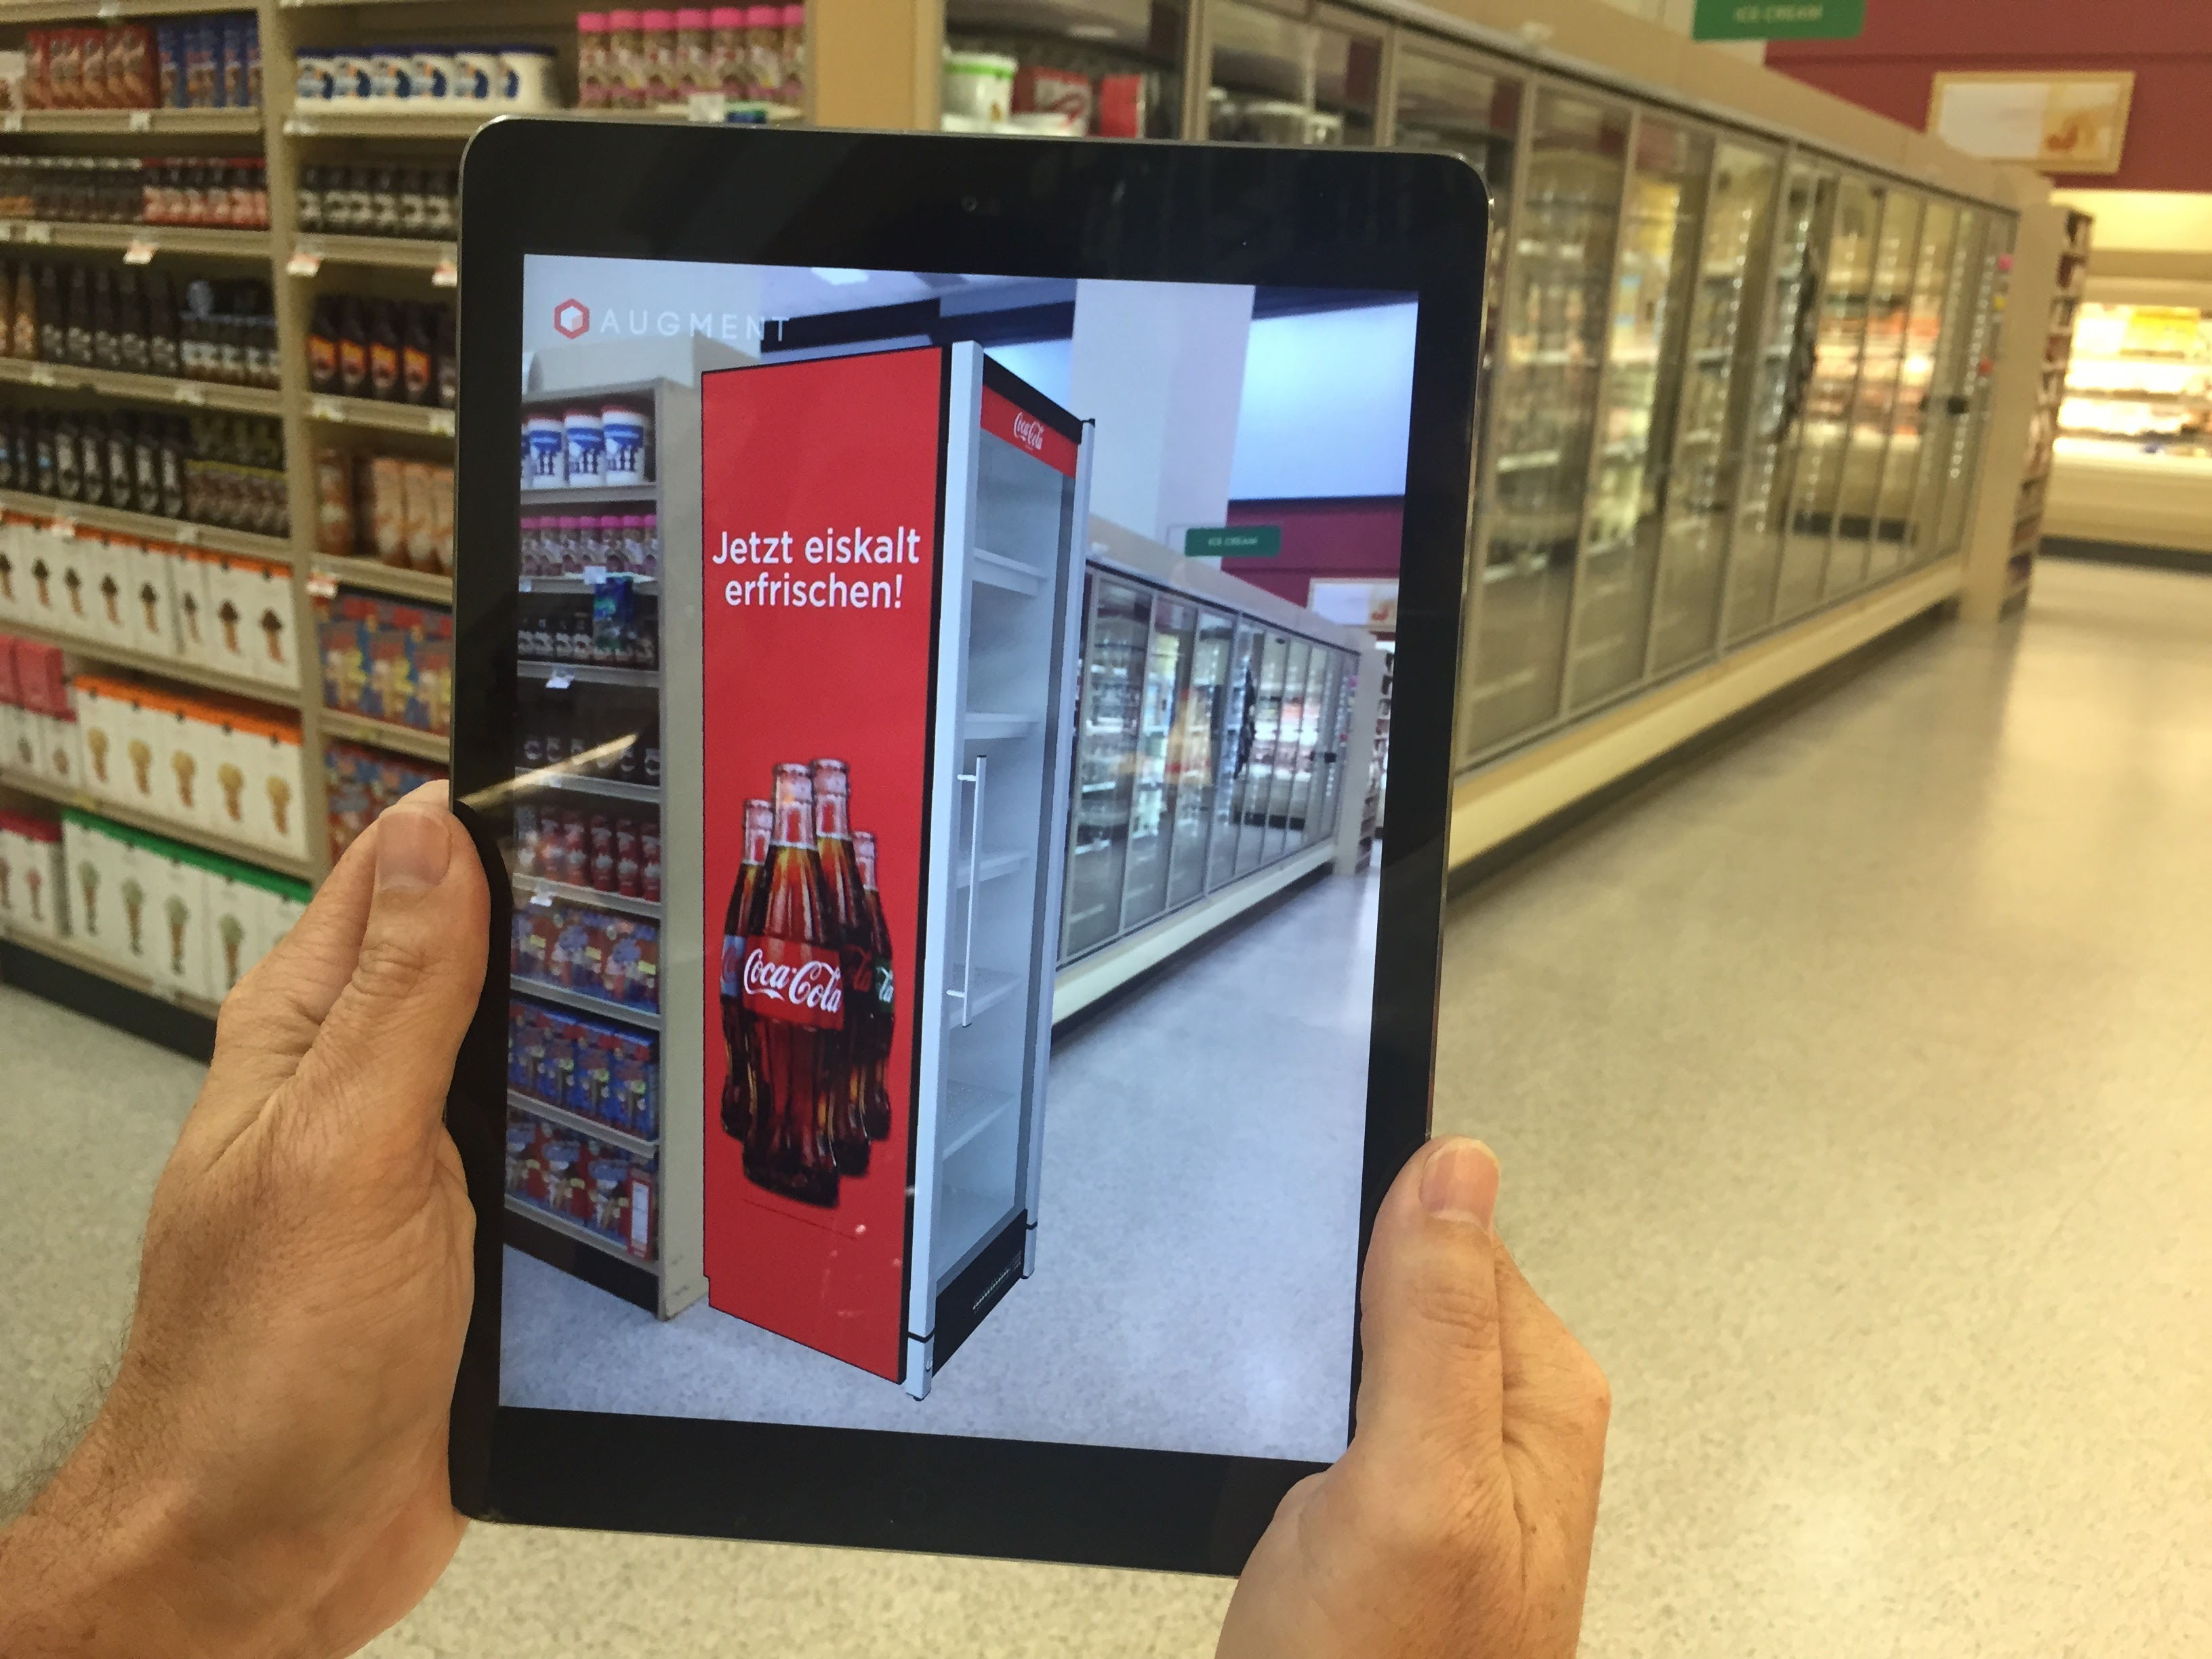
\includegraphics[scale=0.045]{augmentFoto.jpg}
\caption{Augment project met Coca Cola \citep{augmentFoto}}
\vspace{-15pt}
\end{wrapfigure}

Augment werkte al samen met grote bedrijven als Siemens, Coca-Cola en GDF Suez.  Hun focus ligt naast retail ook op educatie. In het verleden werkte Augment ook al nauw samen met universiteiten aan bepaalde projecten. Hun mobiele applicatie is gratis en een account voor modellen te kunnen uploaden isbetalend. Augment biedt gratis licenties voor educatieve doeleinden binnen onderwijsinstellingen. Zowel studenten als leerkrachten kunnen een licentie aanvragen. De mobiele Augment applicatie is al meer dan 2 miljoen keer gedownload en het platform heeft meer dan 10000 gebruikers per dag \citep{augmentData}.




\chapter{Augmented Reality in onderwijs}

In het verleden was de hardware nodig voor Augmented Reality vaak omslachtig, groot en lomp: head-mounted displays, sterke en zware computers of grote projectoren. Dit cre\"eerde ongemakken voor zowel leerlingen als leerkrachten \citep{kerawalla2006}. Nu Augmented Reality alom beschikbaar is op handhelds en handhelds meer en meer ge\"integreerd raken op scholen, zou Augmented Reality veel aantrekkelijker kunnen zijn voor het onderwijs. 

	\section{ICT in het Vlaams onderwijs }
		
	\subsection{Belang}
	Meer dan ooit is ICT overal aanwezig. We leven in een digitaal tijdperk waarin technologie razendsnel evolueert. ICT raakt meer en meer ge\"integreerd in onze samenleving. Het onderwijs kan niet achterblijven. Nieuwe technologi\"en kunnen niet alleen bijdragen aan het bevorderen van de lessen maar het is ook belangrijk dat de leerlingen de nodige vaardigheden ontwikkelen om te voldoen aan de verwachtingen van de arbeidsmarkt en het hoger onderwijs op vlak van ICT-vaardigheden. Daarom stelde de vlaamse overheid de eindtermen op voor ICT, besproken in \ref{sec:eindtermen}.
	
	Het onderwijs kan ook bijdragen op het vlak van technologische kansenongelijkheid. Zo heeft niet iedere leerlingen toegang tot dezelfde toestellen of technologiën als anderen. Dergelijke leerlingen verdienen ook de kans om ICT-vaardigheden onder de knie te krijgen en begeleid te worden in het halen van de eindtermen ICT.
		
	
  \subsection{Eindtermen ICT}
	\label{sec:eindtermen}

	De eindtermen voor onderwijs in Vlaanderen zijn publiekelijk beschikbaar op \\	\href{url}{http://www.ond.vlaanderen.be/}. Eindtermen zijn minimumdoelen op het vlak van kennis, inzicht, vaardigheden en attitudes die de overheid als noodzakelijk en bereikbaarbaar achten voor een bepaalde leerlingenpopulatie \citep{eindtermen}. De ICT eindtermen voor het lager onderwijs gelden als volgt: 
	
	\begin{itemize}
	  \item De leerlingen hebben een positieve houding tegenover ict en zijn bereid ICT to gebruiken om hen te ondersteunen bij het leren.
		\item De leerlingen gebruiken ICT op een veilige, verantwoorde en doelmatige manier.
		\item De leerlingen kunnen zelfstandig oefenen in een door ICT ondersteunde leeromgeving.
		\item De leerlingen kunnen zelfstandig leren in een door ICT ondersteunde leeromgeving.
		\item De leerlingen kunnen ICT gebruiken om eigen ideeën creatief vorm te geven.
		\item De leerlingen kunnen met behulp van ICT voor hen bestemde digitale informatie opzoeken, verwerken en bewaren.
		\item De leerlingen kunnen ICT gebruiken bij het voorstellen van informatie aan anderen.
		\item De leerlingen kunnen ICT gebruiken om op een veilige, verantwoorde en doelmatige manier te communiceren.
	\end{itemize}
	 Deze eindtermen zijn voor het eerst opgesteld zijn in 1997 en zijn in op 1 september 2007 in een nieuw jasje gestoken \citep{besluitEindtermen}. Toen waren tablets en smartphones nog niet zo ge\"integreerd als tegenwoordig. De eindtermen zijn echter actueler dan ooit door de ongelofelijke populariteit van handhelds sinds de release van de iPad in 2010 \citep{choi2013strategic}. Het gebruik van handhelds in de les kan het onderwijs enkel ten goede komen om de leerlingen te helpen deze eindtermen te behalen. \\
	
 Er wordt dus verwacht van de leerlingen dat ze ICT kunnen gebruiken voor allerhande taken in het dagelijks leven. Veilig op het internet surfen, naar juiste en betrouwbare informatie zoeken of het correct gebruiken van een toestel zijn allemaal voorbeelden van vaardigheden die aangeleerd moeten worden.\\

In Vlaamse basis scholen blijkt het dat ondanks de pogingen van de regering om in alle scholen ICT werkelijk in de lessen te integreren,  dit heel sterk af hangt van het beleid van school. Door de grote onafhankelijkheid die Vlaamse scholen krijgen, kan het beleid sterk verschillen tussen scholen. \citep{tondeur2007curricula}. Een tekort aan gebruik van ICT in de lessen is vaak te wijten aan een slechte communicatie tussen directie en leerkrachten \citep{tondeur2007curricula}. 


  \subsection{Handhelds in het Vlaams onderwijs}
	
	In 2012 werd een middelbare school in Blankenberge, Sint-Pieterscollege/Sint-Jozefs handelschool, als eerste Vlaamse school een iPadschool \citep{bettina}. Het concept lijkt populairder in Nederland, waar ook al veel basisscholen een iPadschool zijn geworden \citep{ipadschool}. Sinds de omschakeling van de school in Blankenberge is nog geen andere school in Belgi\"e gevolgd. In een iPadschool is iedere leerling en leerkracht verplicht om een iPad aan te schaffen. Uit het onderzoek van \cite{bettina} bleek dat de integratie van tablets in de school goed te verlopen. Ondanks nog enkele nadelen zoals een klein aanbod cursusmateriaal op de iPad en technische problemen waren de leerlingen en leerkrachten zeer enthousiast. \\
	
	Concrete cijfers over hoeveel scholen wel of niet met handhelds werken zijn er momenteel niet. Wel zijn er aanwijzingen dat heel wat scholen toch tablets beschikbaar stellen voor hun leerlingen en leerkrachten. Zo onderzocht \cite{tabletsOnderwijs} het gebruik van tablets in 16 Vlaamse basisscholen. Hij liet leerlingen oefeningen op tafels maken zowel op een tablet als op papier. Op papier maakten de leerlingen minder fouten en hadden ze minder tijd nodig dan de leerlingen die de oefingen maakten op tablet. Aan de andere kant vonden de leerlingen het wel veel aangenamer en fijner werken op de tablet. Van Gorp concludeert dat tablets zeker een meerwaarde kunnen bieden aan het onderwijs maar dat het een doordachte keuze moet zijn. Een tablet kan ook gebruikt worden als extra motivatie voor de leerlingen. 
	
	

	
\section{Waarom Augmented Reality in onderwijs?}


\subsection{Doelen}
\label{sec:doelen}

Er zijn verschillende manieren waarin AR zijn steentje kan bijdragen in het onderwijs.  Volgens \cite{aredu} zijn er enkele doelen waarin Augmented Reality uitblinkt. Deze doelen zijn echter niet uniek voor Augmented Reality en er zijn veel andere manieren waarop deze gerealiseerd kunnen worden. 

\subsubsection{Leren met 3D-perspectieven \& het onzichtbare tonen}
Met AR kunnen eenvoudig 3D modellen getoond worden. De leerlingen kunnen dan getoonde modellen inspecteren en manipuleren waarbij er extra informatie extra op het scherm kan komen. \cite{wu2001promoting} onderzochten of virtuele modellen konden helpen om studenten chemische structuren beter te doen verstaan. De conclusie was dat de virtualisatie effectief een meerwaarde had voor bepaalde studenten maar dat sommigen nog steeds de voorkeur gaven aan de klassieke re\"ele modellen. Ook een ander onderzoek \citep{chen2011use} kwam tot de conclusie dat werken met AR verrijkend kan zijn, maar de beste resultaten behaald werden door leerlingen die zowel de virtuele als re\"ele modellen gebruikten tijdens het leren. Virtualisaties kunnen ook helpen met het uitleggen van fenomen die niet gezien kunnen worden zoals electromagnetische velden of de werking van ons zonnestelsel. Augmented Reality kan dus aan lessen een perfecte ondersteuning bieden door het integreren van 3D modellen in een les.

\subsubsection{Collaboratief en interactief leren}
Met AR kunnen activiteiten worden uitgewerkt waarbij leerlingen samen kunnen werken op een interactieve manier. Vaak komen deze in een soort van spelvorm waarbij leerlingen op pad gaan buiten de klas. \cite{squire2007augmented} maakten het educatief spelletje Evironmental Detectives waarbij leerlingen met handhelds op onderzoek gingen om een fictieve chemische vervuiling in de nabijgelegen natuur te onderzoeken. Leerlingen kwamen op een realistischere manier in contact met de problemen en leerden zo om beter ge\"informeerde beslissingen te maken door samenwerking en onderzoek. AR kan dus ook gebruikt worden om studenten met elkaar opdrachten te laten uitwerken en op een zelfstandige manier te leren werken. Ondertussen zijn er al applicaties en tools zoals ARLearn die ondersteuning bieden naar uitwerking van dergelijke educatieve spellen voor leerkrachten \citep{arlearn}.

%\subsection{Mobiel leren en games in educatie?}


%nog bijvoegen? 
%http://www.ifets.info/journals/19_1/22.pdf

\subsection{Motivatie}
Een belangrijke factor in het onderwijs is motivatie. In onze samenleving is het normaal dat we een groot deel van ons leven op school spenderen. Een grote uitdaging voor leekrachten is om hun leerlingen te motiveren. Een gemotiveerde leerling werkt beter mee, gedraagt zich beter en haalt uiteindelijk ook betere resultaten.\citep{deci1991motivation}, \citep{theall1999have}.\\

\begin{figure}[h]
\begin{center}
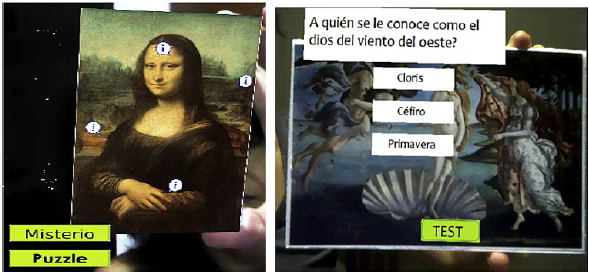
\includegraphics[scale=0.5]{kunst.png}
\caption{AR puzzel en quiz op kunst \citep{di2013impact}}\label{fig:kunst}
\end{center}
\end{figure}


De impact van AR op motivatie werd onderzocht door \cite{di2013impact}. In deze studie werd een les kunstgeschiedenis gegeven op twee manieren aan 69 leerlingen tussen 13 en 16 jaar oud. De les ging over renaissance kunst in Itali\"e.  De eerste manier was een tradionele les met slides en cursus. De tweede manier was een interactieve sessie met Augmented Reality op handhelds waarbij de leerlingen de kunst werd getoond met extra informatie, vragen of beelden zoals getoond in figuur \ref{fig:kunst}. Na beide lessen werden discussiegroepen gehouden. De motivatie van de studenten werd gemeten volgens de IMMS. De onderzoekers concludeerden dat de lessen met AR de studenten wel degelijk meer motiveerde dan de traditionele les. Ook achteraf in de discussies waren de leerlingen die de AR les hadden gekregen veel actiever en praatzamer over de leerstof dan de leerlingen uit de gewone les. De grotere motivatie was te danken aan enkele redenen. Zo was in de tradionele les interactie met de leerstof enkel mogelijk via de leerkracht. Via de AR les hadden de leerlingen zelf controle over het verkennen van de leerstof. De AR les zorgde voor meer interesse en een betere attentiespanne. Ook \cite{solak2015exploring} onderzochten de invloed van AR op onderwijs. Zij spitsten zich toe op vocabularium lessen aan eerstejaars studenten. Ook zij vonden dat Augmented Reality een positieve invloed kan hebben op de motivatie van de leerlingen en bijgevolg de behaalde resultaten beter zijn.
	
\subsection{Vaardigheden}
\label{sec:vaardigheden}
Door het werken met Augmented Reality kunnen leerlingen een waaier van vaardigheden aanleren die in een normale leeromgeving niet aan bod zouden komen. Voorbeelden zijn ruimtelijk inzicht, omgaan met technologie, omgaan met informatie, probleem oplossend denken, samenwerken, zelfstandig leren, ... Welke vaardigheid ontwikkeld wordt hangt af van de specifieke AR toepassing, de activiteit en uiteraard ook de leerstof. Als de activiteit gebruikt maakt van 3D-modellen in AR dan leren de leerlingen deze objecten op een innovatieve manier kennen en oefenen ze hun ruimtelijk inzicht \citep{aredu}. AR in de vorm van een spel zoals Environmental Detectives leert de leerlingen om data te interpreteren en analyseren alsook probleem oplossend te denken \citep{squire2007augmented}.\\

Ook kan Augmented Reality helpen de leerlingen de eindtermen van de Vlaamse Overheid omtrent ICT, zoals besproken in sectie \ref{sec:eindtermen}, te behalen. Handheld toestellen vallen onder ICT \citep{eindtermen} en afhankelijk van de opdracht wordt er dan ook rechtstreeks voldaan aan enkele van de opgestelde eindtermen. Zelfstandig oefenen, zelfstandig leren, omgaan met informatie... Augmented Reality past hier perfect in het plaatje.

\subsection{Valkuilen}
Hoewel Augmented Reality zeker en vast zijn bijdrage kan leveren aan het onderwijs, zijn er ook wel enkele mogelijke valkuilen waardoor de meerwaarde teniet zou kunnen gedaan worden. Zo is het belangrijk dat de leerlingen een positieve ervaring opdoen. Hiervoor dienen zowel de hardware als software naar behoren te werken om frustratie te vermijden \citep{dunleavy2009affordances}. Haperingen in beeld, onscanbare codes of gebrek aan internetconnectie zijn drie voorbeelden van mogelijke ergernis. Omdat handhelds steets krachtiger worden, zijn er minder technische problemen te verwachten. Maar dit zal toch steeds een aandachtspunt blijven.\\

Het is ook nodig dat de moeilijkheid van de opdracht in verhouding staat met de ervaring van de leerlingen met de gebruikte technologie \cite{dunleavy2009affordances}. Als een leerling eerst nog moet leren hoe de AR applicatie werkt, terwijl er meteen verwacht wordt dat hij een ingewikkelde taak moet uitvoeren, dan kan hij zich al snel overdonderd voelen en interesse verliezen. Ook een gebrek aan aan essenti\"ele vaardigheden, zoals die vermeld in sectie \ref{sec:vaardigheden}, kan leiden tot een negatieve ervaring voor de leerling \citep{aredu}. Activiteiten moeten dus met zorg worden voorbereid en er kan e begeleiding nodig zijn om de leerlingen een optimale ervaring te geven. \\


\section{Concrete toepassingen}
Ondertussen heeft men voor Augmented Reality op handhelds verschillende en versatiele toepassingen gevonden in het onderwijs. Enkele unieke of toonaangevende toepassingen komen hier aan bod. \\
  
\subsection{Chemie}
\subsubsection{Elements4d}
Elements4D is een initiatief van DAQRI. Met de aangeboden applicatie voor op handhelds kunnen gebruikers trackers scannen van chemische elementen. Zodra de gebruiker de tracker scant kan hij de elementen bij elkaar brengen. Vervolgens is er een interactie tussen deze elementen, maar enkel als deze in werkelijkheid ook zouden interacteren. Hiernaast biedt Elements4D ook hapklare chemie lessen voor zowel het lager, middelbaar als hoger onderwijs \citep{elements4d}. Voorlopig zijn de aangeboden lessen enkel beschikbaar in het Engels.\\

\begin{figure}[!htr]
\begin{center}
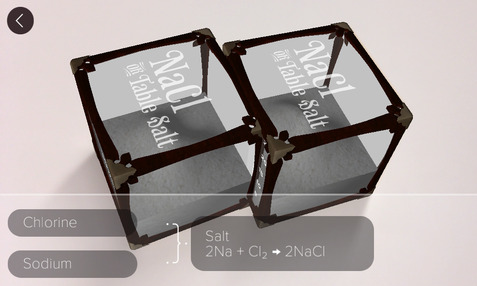
\includegraphics[scale=0.4]{chemie2}
\caption{Interactie tussen atomen met Elements4d \citep{elements4d}}
\end{center}
\end{figure}


\subsubsection{Jonathan Newman}
In de school Rehoboth Christian High School in New Mexico, Verenigde Staten, geeft Jonathan Newman wiskunde en wetenschappen. Sinds Januarie 2016 maakt hij zijn eigen 3D modellen en gebruikt vervolgens Augment om die te kunnen delen met zijn leerlingen \citep{augmentchemie}. Voor het vak chemie gebruikt hij AR om zijn examens op te stellen. Bij de vragen plaatst hij trackers die de leerlingen dan moeten scannen. Op het scherm van hun handhelds komen dan molecules die ge\"identificeerd moeten worden. Ook voor andere doeleinden gebruikt hij AR. In zijn cursus chemie staan ook verscheidene trackers die allerhande modellen of animaties op het scherm tonen. Scan figuur \ref{fig:gas} met de Augment applicatie om te zien hoe moleculen bewegen in een gas.  
\begin{figure}[!htr]
\begin{center}
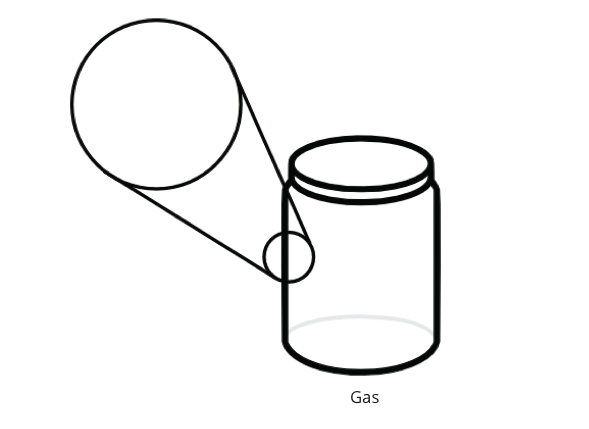
\includegraphics[scale=0.3]{gas}
\caption{Beweging van moleculen in een gas \citep{augmentchemie}} \label{fig:gas}
\end{center}
\end{figure}

\newpage
\subsection{Talen}
\subsubsection{Explorez}
 Voor een case study ontwikkelden \cite{perry2015gamifying} de applicatie Explorez waarbij eerstejaars studenten aan de universiteit van Victoria, Verenigde Staten, via een spel Frans kunnen leren en oefenen. Dit spel is een zoektocht waarbij de leerling de assistent is van een fictief personage dat enkel Frans spreekt. Tijdens de zoektocht maken de studenten interacties mee die getriggerd kunnen worden door middel van locatie, dankzij GPS, of het scannen van QR codes. De interacties omvatten enkele cruciale taalvaardigheden waaronder lezen, schrijven en spreken. Plannen om deze toepassing ook op andere universiteiten te implementeren zijn in de maak \cite{ perry2015gamifying}. Gelijkaardig aan Explorez is er Mentira om Spaans te leren \citep{mentira}.\\

\subsubsection{ChineseCUBES}
ChineseCUBES was een applicatie uitgebracht in 2010 oorspronkelijk enkel op desktop maar later ook op mobile \citep{chinesecubes}. Deze applicatie was gericht op mensen die Chinees wilden leren. De app werkte met kleine vierkante blokken waar telkens Chinese characters op stonden. Deze blokken werden gebruikt voor AR interacties die de gebruiker hielpen om de complexe tekens van het Chinees geschrift aan te leren. Helaas is ChineseCubes onbeschikbaar gesteld. Het bedrijf maakte een laatste tweet eind 2014 \citep{chinesetwitter} maar meer details over waarom hun product niet meer beschikbaar is zijn niet te vinden. \\


\subsection{Overkoepelende applicaties}
\label{sec:overkoepelend}
Er zijn een groot aantal Augmented Reality applicaties te vinden, bruikbaar op handhelds, waarmee leerkrachten aan de slag kunnen om hun lessen te verrijken. Edshelf is een website waarop leerkrachten onder meer applicaties en hun ervaring ermee kunnen delen. Op 22 mei 2016 waren er maar liefst 44 applicaties in de catalogus voor de categorie Augmented Reality \citep{Edshelf}. Er zijn applicaties die basis AR ondersteuning bieden zoals en Augment en Layar maar ook vakspecifieke applicates als Anatomy4D of Elements4D waarmee gebruikers meteen aan de slag kunnen zonder zelf modellen te hoeven uploaden. 

\subsubsection{ARLearn}
ARLearn is een open source en gratis platform dat de kans biedt aan leerkrachten om AR te implementeren in klasuitstappen, zoektochten of andere activiteiten. De voorbereiding gebeurt via een web interface maar voor de uitvoering hebben de deelnemers een mobiele applicatie nodig. ARLearn biedt voorlopig enkel een Android versie aan \citep{arlearn}.\\

\subsubsection{Quiver}
Quiver biedt tekeningen aan die tot leven kunnen komen. In hun gamma zitten zowel gratis als betalende tekeningen. Quiver heeft ook een educatieve bundel. In deze bundel zitten tekeningen die gebruikt kunnen worden in lessen met een educatief doeleinde. Nadat de tekeningen tot leven zijn gekomen zijn er ook interacties mogelijk. Quiver is beschikbaar op zowel Android als iOS \citep{quiver}.
\vspace{10pt}
\begin{figure}[!htr]
\begin{center}
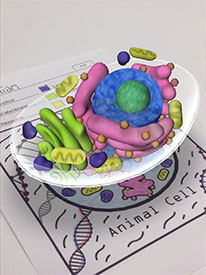
\includegraphics[scale=0.85]{quiver}
\caption{Een tekening tot leven gebracht door \cite{quiver}.}
\end{center}
\end{figure}


\chapter{Case study}
%http://link.springer.com/article/10.1007/s10055-006-0036-4/fulltext.html handig?

 \section{Context}

Daan De Jaeghere is leerkracht lager onderwijs aan het Sint-Andreaslyceum te Sint-Kruis en geeft momenteel les aan het tweede leerjaar. In zijn klas zitten achttien leerlingen van zeven en acht jaar. Daan zocht een manier om een les interactiever en leuker te maken voor de leerlingen en tegelijk gebruik te maken van moderne ICT. Dit is een ideaal scenario om na te gaan of Augmented Reality op handhelds in de les van Daan gebruikt kan worden. \\

In het vak wereldori\"entatie is een van de thema's stoffen. In dit thema leren kinderen over verschillende stoffen: katoen, linnen, wol en zijde. Ze leren waar deze stoffen vandaan komen, wat de eigenschappen zijn en waarvoor ze gebruikt worden. Daan's ervaring is dat dit \'e\'en van de minder leuke onderwerpen is in het vak WO. Door een activiteit te voorzien die gebruik maakt van nieuwe technologi\"en hoopt deze case study de motivatie van de leerlingen op te krikken. In de case study komen zowel de voorbereiding, de uitvoering als de reactie van de leerlingen en de leerkracht aan bod.\\

\section{Methodologie}

\subsection{Voorbereiding}
\label{sec:voorbereiding}
\subsubsection{Infrastructuur}	
De school stelde twee iPads alsook een draadloos netwerk ter beschikking.

\subsubsection{Ervaring van de leerlingen met handhelds}
Om enigzins te kunnen inschatten hoeveel begeleiding er nodig zou zijn voor de leerlingen om met de iPads te kunnen werken, werd er nagegaan wat hun eerdere ervaring met handhelds was. Indien een kind toegang heeft tot een toestel wordt ervan uitgegaan dat zij ervaring hebben met het omgaan van een handheld. Gezien de leeftijd van de kinderen werd volgende vraag aan de ouders gesteld via de agenda: Heeft u kind toegang tot een of meerdere tablet(s) of smartphone(s) thuis? De antwoorden en resultaten zijn te vinden in tabel \ref{table:vraag}.

\begin{table}[h]
\caption{Heeft u kind toegang tot een of meerdere tablet(s) of smartphone(s) thuis?}
\label{table:vraag}
\begin{tabular}{l r}

  &  \\
Mogelijk antwoord & Aantal keer geantwoord\\
\hline
Ja, en mijn kind bezit zelf een tablet en/of smartphone & 7 \\
Ja, maar mijn kind bezit zelf geen tablet en/of smartphone & 5 \\
Neen & 6 \\

\end{tabular}
\end{table}

Elke ouder antwoordde op de vraag. Van de 18 leerlingen is er maar \'e\'en kind op drie dat thuis geen toegang heeft tot een handheld. De anderen hebben thuis wel toegang tot zo'n toestel. \\

\subsubsection{Lesdoelen}
De les moet voldoen aan enkele doelstellingen. De lessen wereldori\"entatie volgen de boeken van Mikado waarin voor de les over stoffen de volgende doelstellingen te vinden zijn \citep{mikado}:
\begin{itemize}
\item Kenmerken van een stof kunnen verwoorden
\item De 4 stoffen correct verwoorden. (Katoen, linnen, wol en zijde)
\item De herkomst van de stof verwoorden. 
\item Samenwerken om tot een consensus te komen.
\item Een stof aanraken en het gevoel beschrijven.
\end{itemize}

Naast deze doelstelling specifiek voor deze les kan het gebruik van handhelds ook bijdragen aan de ICT einddoelen zoals besproken in sectie \ref{sec:eindtermen}. Het Sint-Andreaslyceum is een katholieke school, en ook het katholiek basisonderwijs heeft verschillende doelstellingen rond ICT \citep{katholiek}:
\begin{itemize}
\item leerlingen ontwikkelen kennis, vaardigheden en attitudes met betrekking tot de taal van de media en de vele	toepassingen ervan in de hen omringende wereld met het doel ze te kennen, te begrijpen en te gebruiken.
\item Genoegen (plezier) beleven aan de omgang met media.
\item ...
\end{itemize}

\subsection{Lesvoorbereiding}
\subsubsection{Algemeen}
Aan de hand van de zaken besproken in sectie \ref{sec:voorbereiding} werd de indeling van de les beslist. De leerlingen worden gesplitst in vijf groepen. Deze vijf groepen werken met een doorschuif systeem op vijf verschillende posten. Per stof is er \'e\'en post en om de twintig minuten schuiven de groepjes door. Bij deze posten ligt er stuk stof en is er een invuloefening te maken in het handboek van Mikado. Omdat de snelheid waarmee de oefeningen worden gemaakt kan vari\"eren zijn er kleurplaten, met een AR verrassing, voorzien om de leerlingen op een leuke manier bezig te houden. De vijfde post is een groepsoefening die gebruikt maakt van Augmented Reality op handhelds. Op tafel liggen de vier verschillende stoffen en een aantal afbeeldingen. De leerlingen kunnen deze afbeeldingen scannen met de voorziene iPads waarna er een 3D model op hun toestel verschijnt. Aan de hand van het getoonde model moeten de leerlingen beslissen bij welke stof het voorwerp hoort.\\


\subsubsection{Groepsindeling}
Op basis van de ervaring worden de groepen verdeeld. Voor de klas van achttien leerlingen zijn er drie groepjen van vier en twee groepjen van drie. In de groepen van vier zijn er telkens twee kinderen die zelf een handheld toestel bezitten en twee kinderen die geen toestel thuis hebben. Zo kan er per iPad een ervaren leerling met een onervaren leerling samenwerken waarbij de ervaren leerling dan eventueel uitleg kan voorzien in het gebruik van de iPad. De groepjes van drie bestaan uit de overige leerlingen: vijf met toegang tot een handheld thuis en \'e\'en die zelf een toestel heeft.\\


\subsubsection{AR activiteit}

Op tafel liggen vier stukken stof: katoen, linnen, wol en zijde. Er liggen ook acht afbeeldingen van voorwerpen op de tafel. Deze afbeeldingen zijn afgeprint op hard papier en vervolgens geplastificeerd zodat ze niet snel scheuren of onscanbaar worden. Het groepje leerlingen krijgt eerst een demo waarin ze leren hoe ze een voorwerp kunnen scannen, manipuleren en vervolgens een nieuw voorwerp scannen. In de groepjes van vier werken twee leerlingen samen op \'e\'en iPad en scannen afwisselend. In de groepjes van drie werken de leerlingen per drie met twee iPads. \'E\'en voor \'e\'en scannen de leerlingen de voorwerpen. Terwijl de leerlingen hun kennis delen en overleggen kunnen ze voelen aan de stoffen. Sommige voorwerpen kunnen tot meerde stoffen behoren. De leerlingen hebben normaal gezien al voldoende kennis opgedaan in de voorafgaande WO lessen om de correlaties tussen de voorwerpen en de stoffen te kennen. De gebruikte voorwerpen staan vermeld in tabel \ref{table:models}. Om goed meewerken te stimuleren wordt met een punten systeem gewerkt. Per juist antwoord krijgen de groepen een punt. De groep met het meeste punten mag dan als eerst na de les hun kleurplaten scannen. \\

De criteria voor het slagen van de les zijn:
\begin{itemize}
\item Alle groepen leggen minstens zes afbeeldingen bij een stof.
\item Alle groepen kunnen minstens vier van de acht voorwerpen correct plaatsen.
\item De activiteit moet voor geen enkele groep worden stopgezet om technische redenen.
\item De activiteit moet voor geen enkele groep worden stopgezet door wangedrag van een leerling met behulp van de iPad.
\end{itemize}


\begin{table}[h]
\begin{center}
\label{table:models}
\caption{Gebruikte afbeeldingen en modellen}
\vspace{5pt}
\begin{tabular}{l | l | l}
Afbeelding & Model & Correlatie \\
\hline
Bad & Handdoek & Katoen: neemt goed vocht op \\
Bal wol & Schaap & Wol: komt van de vacht van een schaap\\
Bed & Bed & Linnen: is koel \\
Broek & Broek & Katoen: makkelijk te wassen \\
Plant & Plant & Linnen : komt van een plant \\
      &       & Katoen : komt van een plant \\
Rups & Vlinder & Zijde: zijde komt van een rups \\
Sjaal & Sjaal & Zijde: zijde is zéér zacht \\
 &  &  Wol: is warm \\
Wintermuts & Wollen muts & Wol: is warm \\
\end{tabular}
\end{center}
\end{table}

\subsubsection{3D modellen en afbeeldingen}

De gebruikte afbeeldingen voor de les zijn afkomstig van https://www.pinterest.com/. Alle 3D modellen vanuit de les zijn gratis en publiekelijk beschikbaar op volgende sites:
\begin{itemize}
\item http://archive3d.net/
\item http://tf3dm.com/
\end{itemize}

\subsubsection{Andere activiteiten}
Bij de andere werkposten vullen de leerlingen samen werkblaadjes in over een stof. Deze werkblaadjes komen uit het Mikado handboek \citep{mikado}. Wanneer ze hiermee klaar zijn krijgen ze een Quiver kleurplaat om in te kleuren tot ze kunnen doorschuiven.

\subsubsection{Software}
Voor het scannen en weergeven van de modellen is gekozen om te werken met de Augment applicatie, besproken in sectie \ref{sec:tools}, te werken. Hoewel de applicatie betalend is voorziet Augment gratis licenties aan onderwijsinstellingen. Leerkrachten kunnen dus gratis gebruikt maken van het platform. Ook de functionaliteiten sluiten perfect aan bij het doel van de les. Afbeeldingen scannen en vervolgens een bijhorend 3D model op het scherm toveren is waar Augment zich in specialiseert. Een nadeel aan de applicatie is dat deze niet beschikbaar is in het Nederlands. Dit nadeel valt echter te verwaarlozen mits er bij iedere actie pictrogrammen aanwezig zijn. \\

Voor de kleurplaten werd geopteerd om te werken met Quiver. Deze applicatie is besproken in sectie \ref{sec:overkoepelend}. Quiver heeft als doelgroep zes tot acht jarigen wat de kleurplaten van een gepast niveau maken. Hoewel deze applicatie ook niet in het Nederlands beschikbaar zou dit weinig of geen hinder mogen vormen doordat er een maar en miniem aantal acties zijn. Deze acties zijn dan ook nog eens voorzien van een pictogram. \\

\section{Bevindingen}
De les ging door in het Sint-Andreaslyceum in het lokaal van de klas 2D op dinsdag zeventien mei 2016. Alle achttien leerlingen waren aanwezig. Daan De Jaeghere, leerkracht van de klas, en Thomas Verelst, auteur van deze scriptie, voorzagen begeleiding voor de leerlingen. Er was een leerling jarig. Deze leerling had een snoeptaart mee waardoor de beloning voor de winnende groep steeg: ze mochten ook als eerste hun snoepen kiezen. \\


\subsection{Observaties}

De leerlingen luisterden aandachtig toen hun werd uitgelegd wat de opdracht van de activiteit was en hoe ze met Augment moesten werken. Geen van de leerlingen ondervond technische problemen. In de groepen van vier hielpen de ervaren leerlingen hun onervaren partner zonder dat er ruzie werd vastgesteld. In \'e\'en van de groepjes van drie was er wel discussie ontstaan. Een leerling voelde zich oneerlijk behandeld omdat hij een afbeelding minder mocht scannen, er waren namelijk acht afbeeldingen en drie leerlingen. Dit werd opgelost door de leerling een al behandelde plaat opnieuw te laten scannen. In de tweede groep van drie navigeerde een kind, dat zelf over een iPad beschikt thuis, naar andere applicaties op de iPad waarbij er ingegrepen moest worden. Nadat de leerling erop gewezen was de opdracht te hervatten werden er verder geen problemen meer vastgesteld. De discussies tussen de leerlingen liepen niet uit de hand en ze kwamen telkens samen tot een beslissing over de antwoorden. \\

\begin{wrapfigure}{r}{0.4\textwidth}
\vspace{-10pt}
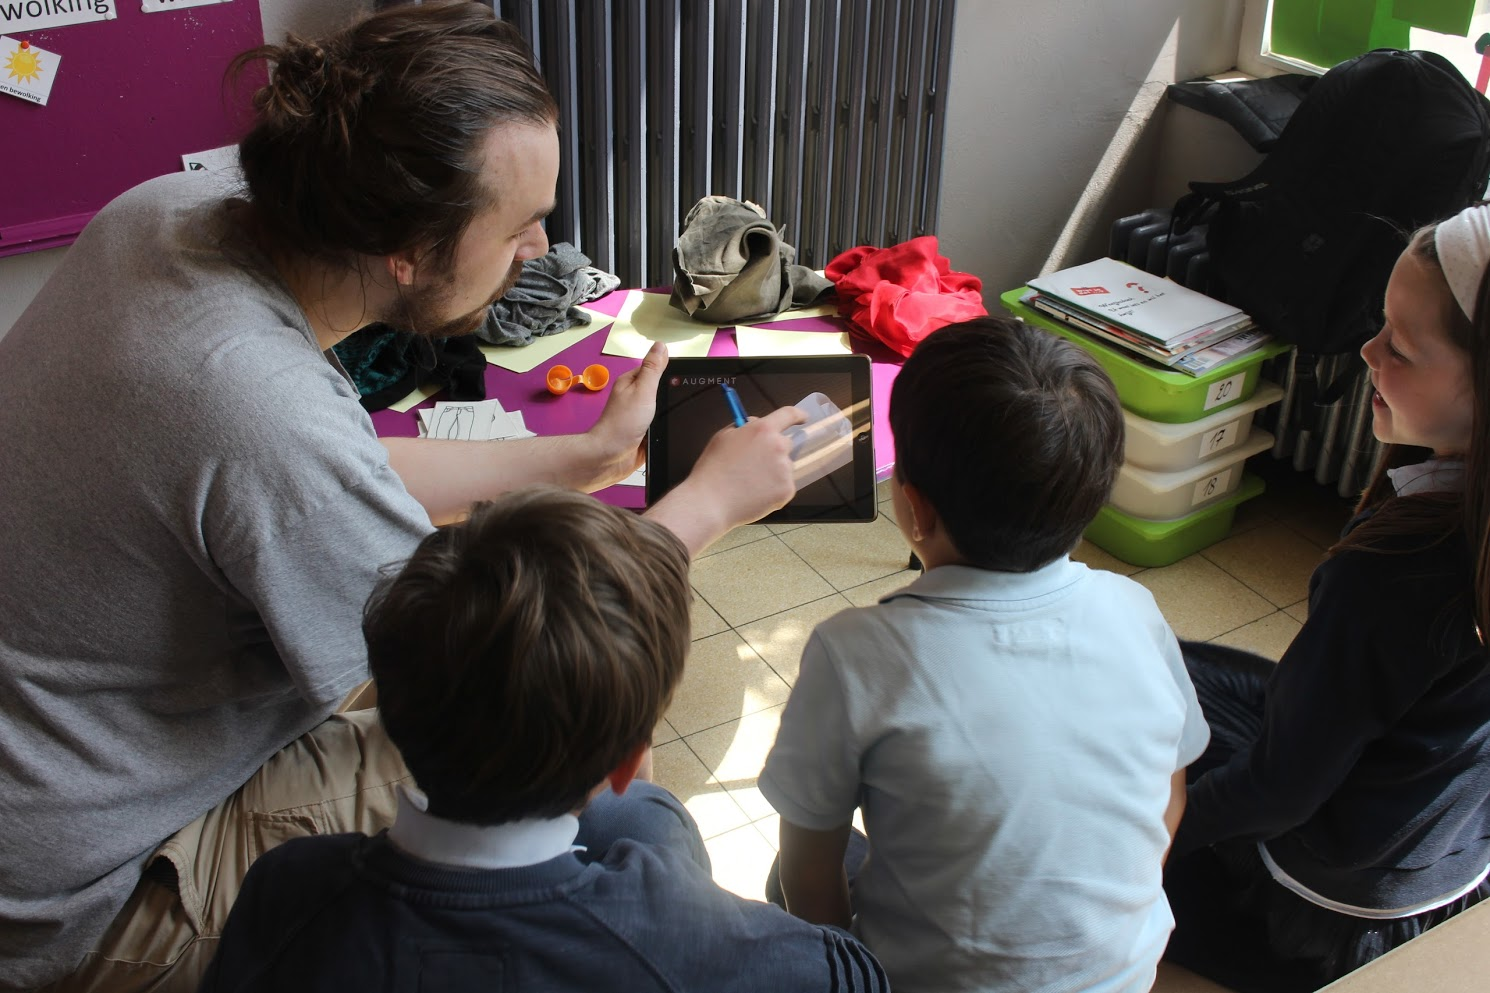
\includegraphics[scale=0.1]{klas1}
\caption{De leerlingen krijgen uitleg}
\end{wrapfigure}

De punten die de groepjes haalden bij de opdracht zijn te vinden in tabel \ref{table:scores}. De gebruikte groepsnummers stemmen overeen met de volgorde waarop ze de activiteit deden. Groep \'e\'en kwam eerst en groep vijf kwam laatst. Groep vier had niet genoeg tijd om alle acht de vragen op te lossen. De andere groepen slaagden er in alle acht de afbeeldingen te klasseren binnen de tijd. Voor geen enkele groep moest de activiteit stopgezet worden en de resultaten voldeden aan de verwachtingen.\\

\begin{table}[h]
\begin{center}
\label{table:scores}
\caption{Punten per groep}
\vspace{5pt}
\begin{tabular}{l | r | r | r}
Groep & \# Leerlingen & Opgelost afbeeldingen & Behaalde punten op 8 \\
\hline
Groep 1 & 4 & 8 & 6 \\
Groep 2 & 4 & 8 & 6 \\
Groep 3 & 4 & 8 & 8 \\
Groep 4 & 3 & 7 & 7 \\
Groep 5 & 3 & 8 & 8 \\
\end{tabular}
\end{center}
\end{table}

De score bij de twee eerste groepen is iets lager dan de andere drie. De verklaring is eenvoudig: de groepen die later kwamen hadden al hun kennis kunnen opfrissen over de verschillende stoffen met de andere opdrachten. \\

Bij de invuloefeningen in de werkboekjes werden geen problemen vastgesteld. De leerlingen werkten samen om de oefeningen te maken. Als de leerlingen klaar waren voordat de twintig minuten verstreken waren konden ze verder kleuren aan hun tekening. Achteraf kregen ze hun kleurplaat mee naar huis. Het was oorspronkelijk de bedoeling dat de tekeningen op het eind van de les gescanned konden worden. Helaas was er door tijdsgebrek geen tijd meer en mochten enkel de leerlingen die thuis  geen handheld ter beschikking hebben hun tekening scannen. De winnende groepen moesten zich tevreden stellen met het eerst kiezen van hun snoepen.

\begin{wrapfigure}{r}{0.3\textwidth}
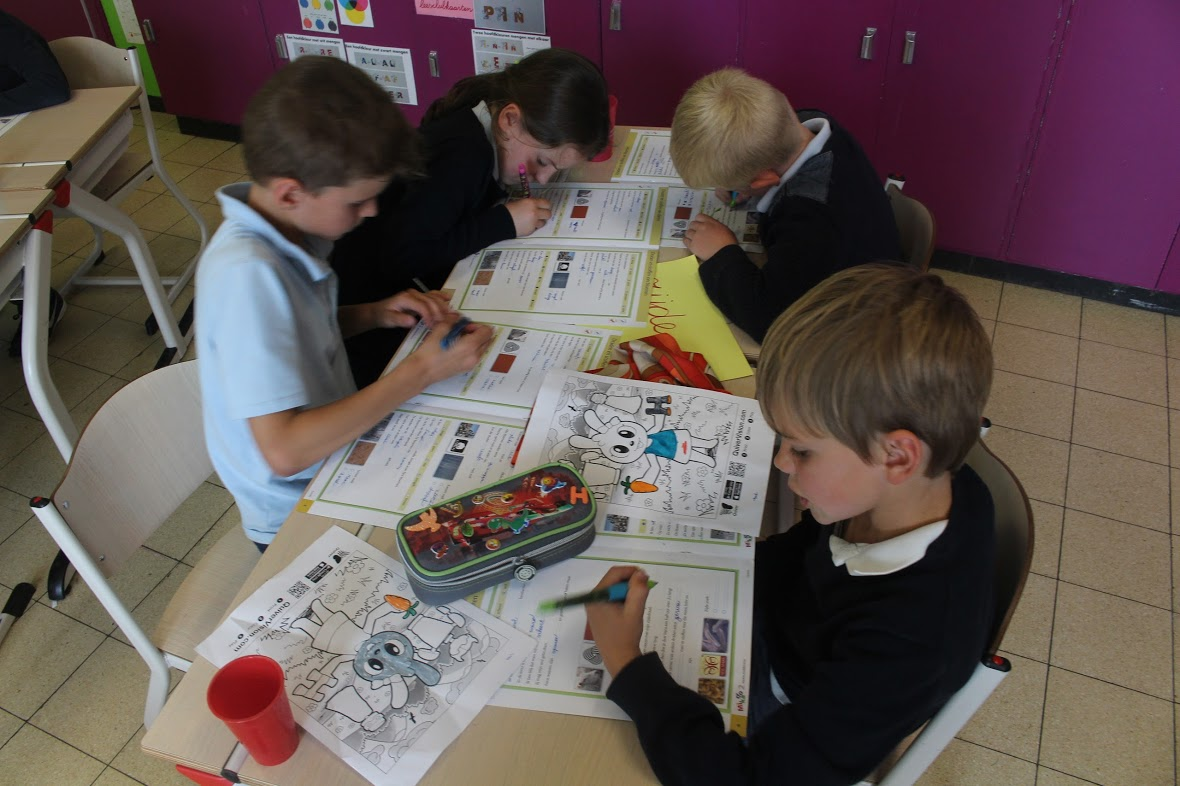
\includegraphics[scale=0.11]{klas2}
\caption{De leerlingen werken aan de invuloefening}
\end{wrapfigure}

\subsection{Reacties}
Om te weten wat de leerlingen van de les vonden werd er een klassikaal gesprek gehouden. Om het gesprek aan te vangen werd er eerst gevraagd wie het de les leuk vond. Vervolgens staken alle leerlingen hun hand in de lucht. Ze kregen de kans om te vertellen waarom ze het een leuke les vonden. Verschillende leerlingen lieten weten dat ze tablets \textit{cool} vonden en dat tablets toffer waren dan een boek. Een vaak vermelde reactie was dat ze liever wat meer tijd hadden gekregen om met de iPad te werken. Hierna werd de vraag gesteld welke leerlingen de les minder leuk vonden. Niemand stak zijn hand op. Ook de leerling die afdwaalde van de opdracht en de leerling die zich benadeeld voelde waren enthousiast.\\ 

Vervolgens werden er drie leerlingen apart genomen voor een gesprek. Van de drie leerlingen was er \'e\'en die thuis zelf een handheld heeft, \'e\'en die een handheld beschikbaar heeft en \'e\'en leerling zonder toegang tot een handheld. Er werd hun gevraagd wat ze van de les vonden en wat er beter kon. Alle drie namen ze ook het woord \textit{cool} in de mond en zeiden ze dat ze het tof vonden om met iPads te werken in de les. Voorgestelde verbeteringen waren dat ze liever langer en ook individueel op de iPad konden werken. Aan deze leerlingen werd ook de vraag gesteld of ze makkelijk konden werken met de applicatie. De leerlingen met ervaring zeiden beiden dat de uitleg voldoende was en dat ze geen problemen hadden. De leerlinge die thuis geen handheld ter beschikking heeft vondt het wel moeilijk maar zei dat ze goed geholpen werd door de leerling waarmee ze samenwerkte. Deze reacties stemmen zijn niet in strijd met de gemaakte observaties. \\

De dag nadien vroeg Daan nogmaals aan zijn leerlingen of er nog opmerkingen of reacties waren. Een leerling liet weten dat hij de activiteit leuk vond deels omdat het een nieuwe manier van werken was, anders dan andere andere dagen. Verder was alle feedback vergelijkbaar met de reacties van de vorige dag. \\ 



Daan was uiterst tevreden over de les: 
\begin{quote}
Ik had er alle vertrouwen in dat de les zou slagen maar ik vreesde dat de leerlingen zich niet zouden focussen op de opdracht. Toen ik ze bezig zag met de iPads was ik trots op mijn leerlingen dat ze zich verantwoordelijk gedroegen. De punten die de groepen scoorden tonen aan dat ze wel degelijk de opdracht maakten en bijgeleerd hebben. De les was geslaagd. De software die we gebruikten wees zichzelf uit en was eenvoudig om mee te werken.
\end{quote}




\subsection{Discussie}

Uit de scores van de groepen en de reacties van de leerlingen kunnen we besluiten dat de les geslaagd was. De vraag blijft wat de rol van Augmented Reality hier nu precies in was. Er konden ook andere manieren zijn om de les interactiever te maken of ICT te integeren zonder AR. De leerlingen zelf leken het meest ge\"interesseerd in de iPads, onafhankelijk van de activiteit. Desondanks boodt AR een goede en leuke ondersteuning voor de les.\\

De leeftijd van de kinderen speelde ook een rol in het verzamelen van reacties. Voor de klassikale discussies was het niet duidelijk of elk kind zijn eigen mening gaf of gewoon de groep volgde. Enkele leerlingen werden apart genomen voor meer persoonlijke feedback. De aanwezigheid van een nieuwe begeleider kon mogelijks de kinderen ge\"intimideerd hebben. Daarom hield Daan nog een klassikaal gesprek de dag nadien.\\

Een van de redenen dat de les vlot en vredezaam verliep is vast en zeker de groepsindeling. Naast de eerder besproken verdeling van de groepen heeft Daan er voor gezorgd dat kinderen, waarvan hij wist dat ze goed overeen komen, in dezelfde groepen terecht kwamen. Doordat er twee begeleiders aanwezig waren kon er \'e\'en de kinderen de uitleg geven voor de AR opdracht terwijl de ander de andere activiteiten in goede banen kon leiden. Ook het feit dat de leerlingen nooit eerder een activiteit in de klas deden op tablets zal bijgedragen hebben aan het enthousiasme.\\

Dat er maar twee iPads ter beschikking waren had zijn voor- en nadelen. Meer tijd per kind op een iPad kon handig geweest zijn. Doordat er maar twee iPads gebruikt werden was het wel eenvoudig om de leerlingen te controleren en ook samenwerking werd hierdoor cruciaal. Door de gelimiteerde tijd bleven de leerlingen ook geboeid tijdens de opdracht en wilden ze hun tijd met de tablet optimaal benutten. De leerlingen hadden geen enkel probleem met het gebruik van de applicatie en dat de voertaal Engels was bleek geen hinder. Dit is duidelijk uit zowel de reacties als het feit dat de leerlingen geen hulp nodig hadden tijdens de opdracht.\\	


%Te jong om notie van AR te hebben? Begeleidbaar door 1 persoon door maar 2 ipads?  3D modellen

\chapter{Conclusie}
\label{ch:conclusie}
%algemeen:
%Veel mogelijkheden, vakspecifiek, niche
%les: niveau goed, tools gratis en beschikbaar: mogelijkheid OK. Begeleiding (door leeftijd?)
%Met de case study is aangetoond dat Augmented Reality wel degelijk in lessen ge\"integreerd kan worden en een positieve ervaring kan 
%resultaten
Augmented Reality is een moderne technologie met enorm veel toepassingen en mogelijkheden. Met de opkomst van de handheld toestellen is de technologie beschikbaar geworden voor iedereen. Er is niet langer robuuste hardware nodig om AR te implementeren. Ook bedrijven is dit niet ontgaan. Er zijn ondertussen tal van bedrijven die zich toespitsen in het verlenen van AR diensten. Naast marketing, retail, kunst, ...  heeft ook in onderwijs Augmented Reality zijn toepassingen gevonden. Doordat ook handhelds in het onderwijs meer en meer ge\"integreerd geraken wordt het ook enkel maar eenvoudiger om de technologie te gebruiken in de lessen. \\

Onderzoek wijst erop dat AR op verschillende manieren nuttig kan zijn in educatie. Zo kan Augmented Reality extra informatie en meerwaarde bieden over de leerstof in kwestie en kan het gebruikt worden om interactieve activiteiten voor te bereiden. AR komt ook de motivatie van de leerlingen ten goede. De leerlingen kunnen een waaier van vaardigheden aanleren met verschillende AR activiteiten.  Wel zijn er enkele valkuilen. Het is belangrijk dat er zo weinig mogelijk technische problemen voorkomen en de gebruikte technologie mag niet te ingewikkeld zijn zodat de leerlingen zich met de opdracht bezighouden. Er moet ook gepaste begeleiding voorzien zijn. \\

Met de case study is aangetoond dat de mogelijkheden bestaan zodat leerkrachten succesvol AR kunnen integreren in hun lessen op handhelds. De activiteit voldeed aan de doelstellingen en de cruciale factoren waren begeleiding, een duidelijk opdracht en eenvoudig te gebruiken software. Uit de observaties en reacties van de leerlingen bleek dat ze de opdracht leuk vonden en ze enthousiast waren. Dit kwam omdat ze op een interactieve manier konden werken met een handheld en de les vernieuwend was. Ook de betrokken leerkracht was tevreden met de implementatie van AR. \\

Augmented Reality op handhelds in het onderwijs staat nog in zijn kinderschoenen, maar toch zijn er al tal van toepassingen en mogelijkheden waarvan leerkrachten kunnen gebruik maken. Naarmate handhelds hun plaats vinden in de klas zal AR ongetwijfeld mee evolueren. \\
%leerkrachten , 


%Veel andere onderzoeken hebben het nut van Augmented Reality al aangetoond. Het kan extra informatie en meerwaarde bieden over de leerstof in kwestie. Het kan evengoed gebruikt worden om interactieve activiteiten voor te bereiden en zo de leerlingen te motiveren. Deze scriptie toont aan dat er mogelijkheden bestaan waarmee leerkrachten AR in hun lessen kunnen integreren op een succesvolle manier. 


\clearpage
\addcontentsline{toc}{chapter}{Literatuur}
\bibliographystyle{apa}
\bibliography{tin-bachproef}



%%---------- Back matter -------------------------------------------------



\clearpage
\addcontentsline{toc}{chapter}{\listfigurename}
\listoffigures


\clearpage
\addcontentsline{toc}{chapter}{\listtablename}
\listoftables

\clearpage
\nomenclature{AR}{Augmented Reality}%
\nomenclature{FPS}{Frames per seconde}%
\nomenclature{ICT}{Informatie en communicatie technologie}%
\nomenclature{IMMS}{Instructional materials motivation survey}%
\nomenclature{QR}{Quick response}%
\nomenclature{SDK}{Software development kit}%
\nomenclature{VR}{Virtual Reality}%
\printnomenclature


\end{document}
